%    Copyright (C) 2012  R. Koller, L. Schmid, S. Eicher
%
%    This file is free: you can redistribute it and/or modify
%    it under the terms of the GNU General Public License as published by
%    the Free Software Foundation, either version 3 of the License, or
%    (at your option) any later version, but you have to reference to the original owner.
%
%	 Additionaly the authors have to be readable in the final document.
%
%    This program is distributed in the hope that it will be useful,
%    but WITHOUT ANY WARRANTY; without even the implied warranty of
%    MERCHANTABILITY or FITNESS FOR A PARTICULAR PURPOSE.  See the
%    GNU General Public License for more details.
%
%    You should have received a copy of the GNU General Public License
%    along with this program.  If not, see <http://www.gnu.org/licenses/>.

%%%%%%%%%%%%%%%%%%%%%%%%%
% Dokumentinformationen %
%%%%%%%%%%%%%%%%%%%%%%%%%

\newcommand{\titleinfo}{Pattern Classification}
\newcommand{\authorinfo}{R. Koller, L. Schmid, S. Eicher} % Do not remove any names! Initial authors stay first.
\newcommand{\versioninfo}{$Revision: 141 $}

%%%%%%%%%%%%%%%%%%%%%%%%%%%%%%%%%%%%%%%%%%%%%
% Standard projektübergreifender Header für
% - Makros 
% - Farben
% - Mathematische Operatoren 
%
% DORT NUR ERGÄNZEN, NICHTS LÖSCHEN
%%%%%%%%%%%%%%%%%%%%%%%%%%%%%%%%%%%%%%%%%%%%%  
% Genereller Header
\documentclass[10pt,twoside,a4paper,fleqn]{article}
\usepackage[left=1cm,right=1cm,top=1cm,bottom=1cm,includeheadfoot]{geometry}
\usepackage[english]{babel}
\usepackage[utf8]{inputenc}

% Pakete
\usepackage{amssymb}
\usepackage{amsmath}
\usepackage{bm}       % Bold Math
\usepackage{fancybox}
\usepackage{graphicx}
\usepackage{color}
\usepackage{lastpage}
\usepackage{wrapfig}
\usepackage{fancyhdr}
\usepackage{hyperref}
\usepackage{verbatim}
\usepackage{pdflscape} % landscape
\usepackage{multirow} % zellen in tabellen verbinden
\usepackage{multicol} 
%\usepackage{slashbox} % getrennte zelle in tabelle
\usepackage{enumitem}
% \usepackage{array} % anordnung in tabellen

%%%%%%%%%%%%%%%%%%%%
% Generelle Makros %
%%%%%%%%%%%%%%%%%%%%
\newcommand{\formelbuch}[1]{$_{\textcolor{red}{\mbox{\small{p. #1}}}}$}
\newcommand{\verweis}[2]{ {\small (siehe auch \ref{#1}, #2 (S. \pageref{#1}))
}}
\newcommand{\subsubadd}[1]{\textcolor{black}{\mbox{#1}}}
\newenvironment{liste}[0]{
	\begin{list}{$\bullet$}{\setlength{\itemsep}{0cm}\setlength{\parsep}{0cm} \setlength{\topsep}{0cm}}}
    {\end{list}}

\newenvironment{beschreibListe}[0]{\vspace{-2mm}
	\begin{description}[noitemsep, nolistsep]\setlength{\itemsep}{0cm} \setlength{\parsep}{0cm} \setlength{\topsep}{0cm} \setlength{\parskip}{0cm}}
    {\end{description}}

    
\newcommand{\logd}[0]{\log_{10}}
\newcommand{\subsubsubsection}[1]{\textbf{#1}}

\newenvironment{aufzaehlung}[0]{
	\begin{enumerate}\setlength{\itemsep}{0cm}\setlength{\parsep}{0cm} \setlength{\topsep}{0cm} \setlength{\parskip}{0cm}} {\end{enumerate}}

\newcommand{\abbHeight}[3]{
	\begin{center}
		\includegraphics[height=#2]{./bilder/#1} \\
		#3
    \end{center}
}

\newcommand{\hilight}[1]{\colorbox{yellow}{#1}}
\newcommand{\todo}[1]{\colorbox{red}{TODO: #1}}

\newcommand{\skriptsection}[2]{\section{\texorpdfstring{#1 \formelbuch{#2}}{#1}}}
\newcommand{\skriptsubsection}[2]{\subsection{\texorpdfstring{#1 \formelbuch{#2}}{#1}}}
\newcommand{\skriptsubsubsection}[2]{\subsubsection{\texorpdfstring{#1 \formelbuch{#2}}{#1}}}
\newcommand{\skriptsubsubsubsection}[2]{\subsubsubsection{\texorpdfstring{#1 \formelbuch{#2}}{#1}}}

%%%%%%%%%%
% Farben %
%%%%%%%%%%
\definecolor{black}{rgb}{0,0,0}
\definecolor{red}{rgb}{1,0,0}
\definecolor{white}{rgb}{1,1,1}
\definecolor{grey}{rgb}{0.8,0.8,0.8}

%%%%%%%%%%%%%%%%%%%%%%%%%%%%
% Mathematische Operatoren %
%%%%%%%%%%%%%%%%%%%%%%%%%%%%
\DeclareMathOperator{\sinc}{sinc}
\DeclareMathOperator{\sgn}{sgn}
\newcommand{\error}{\mathrm{error}}
\newcommand{\bfx}{\mathbf{x}}
\DeclareMathOperator{\expected}{\mathcal{E}}


% Fouriertransformationen
\unitlength1cm
\newcommand{\FT}
{
\begin{picture}(1,0.5)
\put(0.2,0.1){\circle{0.14}}\put(0.27,0.1){\line(1,0){0.5}}\put(0.77,0.1){\circle*{0.14}}
\end{picture}
}


\newcommand{\IFT}
{
\begin{picture}(1,0.5)
\put(0.2,0.1){\circle*{0.14}}\put(0.27,0.1){\line(1,0){0.45}}\put(0.77,0.1){\circle{0.14}}
\end{picture}
}



%%%%%%%%%%%%%%%%%%%%%%%%%%%%
% Allgemeine Einstellungen %
%%%%%%%%%%%%%%%%%%%%%%%%%%%%
%pdf info
\hypersetup{pdfauthor={\authorinfo},pdftitle={\titleinfo},colorlinks=false}
\author{\authorinfo}
\title{\titleinfo}

%Kopf- und Fusszeile
\pagestyle{fancy}
\fancyhf{}
%Linien oben und unten
\renewcommand{\headrulewidth}{0.5pt} 
\renewcommand{\footrulewidth}{0.5pt} 

\fancyhead[L]{\titleinfo{ }- Summary}
%Kopfzeile rechts bzw. aussen
\fancyhead[R]{\today{ }- Page \thepage/\pageref{LastPage}}
\fancyfoot[C]{\copyright{ }\authorinfo}

% Einr�cken verhindern versuchen
\setlength{\parindent}{0pt}



% Möglichst keine Ergänzungen hier, sondern in header.tex
\begin{document} 
 
%%%%%%%%%%%%%%%%%%%%%%%%%%%%%%%%%%%%%%%%%%%%%%%%%%%%%%%%%%%%%%%%%%%%%%%%%%%%%%%%%%%%%%%%%%%%%%%
%%%%%%%%%%%%%%%%%%%%%%%%%%%%%%%%%%%%%%%%%%%%%%%%%%%%%%%%%%%%%%%%%%%%%%%%%%%%%%%%%%%%%%%%%%%%%%%
\section{Bayesian Decision Theory}
\skriptsubsection{Basics}{20}
\begin{minipage}{9.5cm}
  $\{\alpha_1, \ldots \alpha_a\}$ possible actions.
  $\{\omega_1, \ldots \omega_c\}$ 'states of nature' (categories).
  $\mathbf{x}$ is the measurement:
  \begin{center}
    \hilight{$P(\omega_i|x) = \frac{p(x|\omega_i) P(\omega_i)}{p(x)}$} \\
    $= \underbrace{\frac{p(x|\omega_i) P(\omega_i)}{\int\limits_{-\infty}^{\infty}p(x|\omega_j) P(\omega_j) dx}}_{\text{Continous features}}
     \text{ or } 
     \underbrace{\frac{p(x|\omega_i) P(\omega_i)}{\sum\limits_{j=1}^{c}p(x|\omega_j) P(\omega_j)}}_{\text{Discrete features \formelbuch{51}}}$
    \hilight{$ Posterior = \frac{Likelihood \; \times \; Prior}{Evidence}$}
  \end{center}
  
  $$P(error|x) = \int_{-\infty}^{\infty} P(error, x) dx = \int_{-\infty}^{\infty} P(error|x) p(x) dx$$
  $$P(error|x) = \min\Big(P(\omega_1|x), P(\omega_2|x)\Big)$$
  
  
\skriptsubsection{Continuous Features}{24}
The overall risk $R$ must be minimized:
$$R(\alpha_i|\mathbf{x}) = \sum\limits_{j=1}^c \lambda(\alpha_i|\omega_j) P(\omega_j|\mathbf{x})$$
Action: $\alpha(\bm x)$, feature space: $\mathbf{R}^d$; loss or cost function when taking action $i$ 
when the state of nature is $j$: $\lambda(\alpha_i|\omega_j)$
  
\end{minipage} \vspace{1cm}
\begin{minipage}{9cm}
  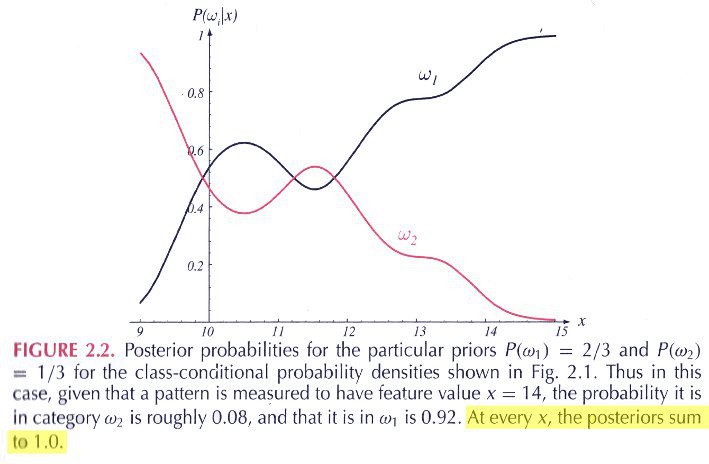
\includegraphics[width=8.5cm]{./images/posterior-prob.jpg}\\
  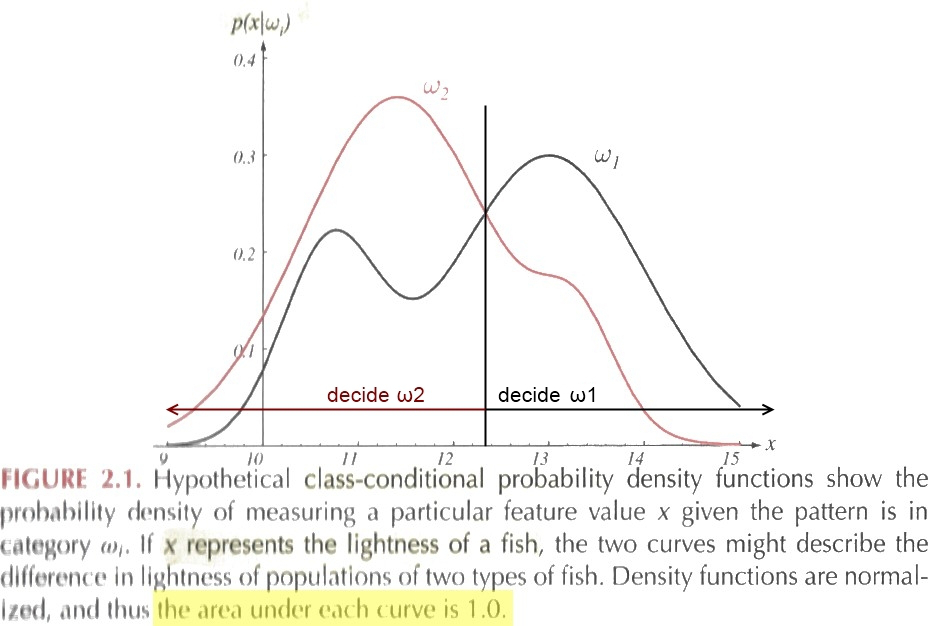
\includegraphics[width=8.5cm]{./images/class-cond-prob.jpg}
\end{minipage}

\skriptsubsection{Two-Category Classification}{25}
Decide $\omega_1$ when
$$\frac{p(\mathbf{x}|\omega_1)}{p(\mathbf{x}|\omega_2)} > \underbrace{
\frac{\lambda_{12} - \lambda_{22}}{\lambda_{21} - \lambda_{11}} \frac{P(\omega_2)}{P(\omega_1)}}_{\text{constant}}$$
where $\lambda_{12}$, $\lambda_{21}$ are the costs for a wrong decision and 
$\lambda_{11}$, $\lambda_{22}$ for the correct decision (which are usually $0$).

\skriptsubsection{Classifiers}{29}
\subsubsection{Multicategory Case}
Discriminant functions: $g_i(\mathbf{x}) > g_j(\mathbf{x})$ for all $j \neq i$
$$g_i(\mathbf{x}) = P(\omega_i|x) = 
\frac{p(x|\omega_i) P(\omega_i)}{\sum\limits_{j=1}^{c}p(x|\omega_j) P(\omega_j)}$$

\subsubsection{Two-Category Case}
Decide $\omega_1$ when $g(\mathbf{x}) > 0$:
$$g(\mathbf{x}) \equiv g_1(\mathbf{x}) - g_2(\mathbf{x})\hspace{5mm} \text{ or } \hspace{5mm}  
g(\mathbf{x}) = \ln \frac{p(\mathbf{x}|\omega_1)}{p(\mathbf{x}|\omega_2)} + \ln \frac{P(\omega_1)}{P(\omega_2)}$$


\skriptsubsection{Normal Density}{31}
  \skriptsubsubsection{Univariate Density}{32}
  \begin{minipage}{12cm}
  Viele kleine, unabhängige Zufallsvariable sammeln sich zu einer
  normalverteilten Zufallsvariable.\\
   $\varphi(x)=p(x)=\frac{1}{\sqrt{2
  \pi}\sigma}\cdot e^{-\frac{(x-\mu)^2}{2\sigma^2}} = N(\mu ; \sigma^2) \qquad \mu=E(x)=\int\limits_{-\infty}^{\infty}{x p(x) dx}$\\ 
  $F(x)=\frac{1}{\sqrt{2
  \pi}\sigma}\cdot \int\limits^{x}_{-\infty}{e^{-\frac{(\tilde{x} -\mu)^2}{2\sigma^2}}} \qquad \sigma^2=E\left[(x-\mu)^2\right]=\int\limits_{-\infty}^{\infty}{(x-\mu)^2 p(x) dx}$ \\
  % = N(\mu ; \sigma^2),\tilde{x}} $
  \textbf{Standardisierung}\\
  Erwartungswert: $E(X)=\mu$ \hspace{4mm}(=0 bei Standardnormalver.)\\ 
  Varianz \hspace{11.5mm}: $var(X)=\sigma^2$ (=1 bei Standardnormalver.)\\ \\
  $x=\dfrac{X-\mu}{\sigma}$ \hspace{5mm} $x$ aus Tabelle
  \end{minipage}
  \begin{minipage}{7cm}
  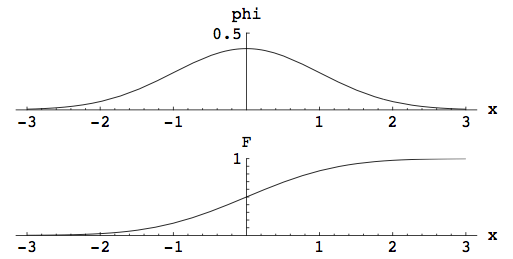
\includegraphics[width=7cm]{../WrStat/bilder/normalverteilung.png}
  Dichtefunktion (oben) und Verteilungsfunktion (unten) der Normalverteilung. 
  \end{minipage} \\ \\ 
 $ 68\% $ der Werte liegen im Intervall $[ \mu - \sigma, \mu + \sigma]$, $95\% $ in $[ \mu - 2\sigma, \mu + 2\sigma]$, $99.7\% $ in $[ \mu - 3\sigma, \mu + 3\sigma]$



\skriptsubsubsection{Multivariate Density}{33}
  $N(\boldsymbol{\mu}, \boldsymbol{\Sigma}) \backsim p(\mathbf{x}) = \frac{1}{(2\pi)^{d/2} | \boldsymbol{\Sigma}|^{1/2}} \exp \bigg[-\frac{1}{2} (\mathbf{x} - \boldsymbol{\mu})^T \boldsymbol{\Sigma}^{-1} (\mathbf{x}-\boldsymbol{\mu})\bigg]$
  \\
  \subsubsubsection{The whitening transform} leads to a proportional matrix of the identity matrix $\mathbf{I}$:
  $\mathbf{A}_w = \boldsymbol{\Phi} \boldsymbol{\Lambda}^{-1/2}$ 
  where $\mathbf{\Phi}$ is matrix whose columns are the orthonormal eigenvectors of 
  $\mathbf{\Sigma}$ and $\mathbf{\Lambda}^{1/2}=\begin{bmatrix}
  \sqrt{\lambda_1}& 0 & \ldots \\
  0&\sqrt{\lambda_2}&\ldots\\
  \ldots
  \end{bmatrix}$ its eigenvalues.
  
  \subsubsubsection{Mahalanobis Distance} from $\mathbf{x}$ to $\boldsymbol{\mu}$: $r^2 = (\mathbf{x}-\boldsymbol{\mu})^T \boldsymbol{\Sigma}^{-1} (\mathbf{x}-\boldsymbol{\mu})$ 
  is with the co-/ variance ``normalized'' distance from the given point to the mean.
  
  
  \subsubsection{Covariance}  
  Covariance: $\sigma_{xy} = c_{xy}= \operatorname{Cov}(X,Y) = E((x-E(X))(y-E(Y))) = E(XY^*)-E(X)E(Y)= \underbrace{0}_{\text{falls X,Y unabhängig}}= \underbrace{r_{xy}}_{\text{falls X,Y mittelwertsfrei}}$
  \\
  Covariance matrix: $\operatorname{Cov}(X) = \mathbf{\Sigma} = 
  \bigl(\operatorname{Cov}(X_i, X_j)\bigr)_{i,j=1,\ldots,n} = \begin{pmatrix} 
\operatorname{Cov}(X_1,X_1) & \cdots & \operatorname{Cov}(X_1,X_n) \\
\vdots & \ddots & \vdots \\
\operatorname{Cov}(X_n,X_1) & \cdots& \operatorname{Cov}(X_n,X_n)\end{pmatrix}$\\


  \skriptsubsubsection{Discriminant Functions for the Gaussian Density}{36}
  \label{sec:bayes_discriminant_function}
  \subsubsubsection{Case 1: $\Sigma_i = \sigma^2 I$}\\
  Same variance in all independent features.
  The linear discriminant function turns to: 
  $$g_i(\mathbf{x}) = \mathbf{w}_i^T \mathbf{x} + w_{i0} \text{ with } 
  \mathbf{w}_i = \frac{1}{\sigma^2}\boldsymbol{\mu}_i \text{ and }
  w_{i0} = -\frac{1}{2\sigma^2} \boldsymbol{\mu}_i^T \boldsymbol{\mu}_i + \ln(P(\omega_i))$$
  
  The decision surface is a plane: $\mathbf{w}^T(\mathbf{x}-\mathbf{x}_0) = 0$ with $\mathbf{w} = \boldsymbol{\mu}_i - \boldsymbol{\mu}_j$ and 
  $\mathbf{x}_0 = \frac{1}{2}(\boldsymbol{\mu}_i-\boldsymbol{\mu}_j) - \frac{\sigma^2}{||\boldsymbol{\mu}_i-\boldsymbol{\mu}_j||^2} \ln\left(\frac{P(\omega_i)}{P(\omega_j)}\right) (\boldsymbol{\mu}_i-\boldsymbol{\mu}_j)$
  
  
  \subsubsubsection{Case 2: $\Sigma_i = \Sigma$}\\
  Some covariance matrix for all classes.
  The linear discriminant function turns to: 
  $$g_i(\mathbf{x}) = \mathbf{w}_i^T \mathbf{x} + w_{i0} \text{ with } 
  \mathbf{w}_i = \boldsymbol{\Sigma}^{-1}\boldsymbol{\mu}_i \text{ and }
  w_{i0} = -\frac{1}{2} \boldsymbol{\mu}_i^T \boldsymbol{\Sigma}^{-1}\boldsymbol{\mu}_i + \ln(P(\omega_i))$$
  
  The decision surface: $\mathbf{w}^T(\mathbf{x}-\mathbf{x}_0) = 0$ with $\mathbf{w} = \boldsymbol{\Sigma}^{-1} (\boldsymbol{\mu}_i - \boldsymbol{\mu}_j)$ and 
  $\mathbf{x}_0 = \frac{1}{2}(\boldsymbol{\mu}_i-\boldsymbol{\mu}_j) - \frac{\sigma^2}{(\boldsymbol{\mu}_i-\boldsymbol{\mu}_j)^T \boldsymbol{\Sigma}^{-1} (\boldsymbol{\mu}_i-\boldsymbol{\mu}_j)} \ln\left(\frac{P(\omega_i)}{P(\omega_j)}\right) (\boldsymbol{\mu}_i-\boldsymbol{\mu}_j)$
  
  
  \subsubsubsection{Case 3: $\Sigma_i = $ arbitrary}\\
  General case.
  The discriminant function is now quadratic: 
  $$g_i(\mathbf{x}) = \mathbf{x}^T \mathbf{W}_i^T \mathbf{x} + \mathbf{w}_i^T \mathbf{x} +w_{i0} \text{ with } 
  \mathbf{W}_i = -\frac{1}{2} \boldsymbol{\Sigma}^{-1} \text{ and }
  \mathbf{w}_i = \boldsymbol{\Sigma}^{-1}\boldsymbol{\mu}_i \text{ and }
  w_{i0} = -\frac{1}{2} \boldsymbol{\mu}_i^T\boldsymbol{\Sigma}^{-1}\boldsymbol{\mu}_i - \frac{1}{2}\ln(|\boldsymbol{\Sigma}_i|) + \ln(P(\omega_i))$$
  
  The decision surface cannot be described easily anymore as it may contain holes and nonlinear constructions.
  
  Example: \formelbuch{44}
  

\skriptsubsection{Independent Binary Features}{52}
  Every component $x_i$ of vector $\mathbf{x}$ are either 0 or 1. The class-conditional probability is:\\
  $$P(\mathbf{x}|\omega_1)=\prod\limits_{i=1}^d p_i^{x_i}(1-p_i)^{1-x_i} \qquad ( p_i^{x_i}(1-p_i)^{1-x_i} \Rightarrow\text{ either }p_i\text{ or }1-p_i)$$
  
  Discriminant function: $g(\bm x) = \sum\limits_{i=1}^d w_i x_i + w_0$ with 
  $w_i = \ln \frac{p_i(1-q_i)}{q_i(1-p_i)}$ and 
  $w_0 = \sum\limits_{i=1}^d \ln \frac{1-p_i}{1-q_i} + \ln \frac{P(\omega_1)}{P(\omega_2)}$
  
  Example: \formelbuch{53}
\skriptsection{Maximum-Likelihood and Bayesian Parameter Estimation}{84}

  \skriptsubsection{Maximum-Likelihood Estimation (ML)}{85}
  Maximum-Likelihood estimation tries to find an optimum solution if a parameter vector
  $\boldsymbol{\theta}$ is unknown.
  The likelihood of $\boldsymbol{\theta}$ with respect to the set of samples $\mathcal{D}$ is defined as 
  $p(\mathcal{D} | \boldsymbol{\theta}) = \prod_{k=1}^{n} p(\mathbf{x}_k | \boldsymbol{\theta})$ 
  (samples are i.i.d. - independent \& identically distributed).
  
  \begin{minipage}{12cm}
	  Recipe with log-likelihood: \\
	  \begin{tabular}{lll}
	  1. & Log-likelihood: & $l(\boldsymbol{\theta}) \equiv \ln (p(\mathcal{D} | \boldsymbol{\theta}))=\sum\limits_{k=1}^n \ln(p(\mathbf{x}_k | \boldsymbol{\theta}))$ \quad $\left( \frac{d}{dx} \ln(x) = \frac1x \right)$ \\
	  2. & Gradient: &  $\nabla_{\boldsymbol{\theta}} l = 
	  	      \sum\limits_{k=1}^n \nabla_{\boldsymbol{\theta}}\ln(p(\mathbf{x}_k | \boldsymbol{\theta}))$ \\
	  3. & $\nabla_{\boldsymbol{\theta}} l = 0$: & find solution 
	  	      $\boldsymbol{\hat{\theta}}=\arg\max\limits_{\boldsymbol{\theta}} l(\bm{\theta})$ \\
	  \end{tabular}
  \end{minipage}
  \begin{minipage}{8cm}
  	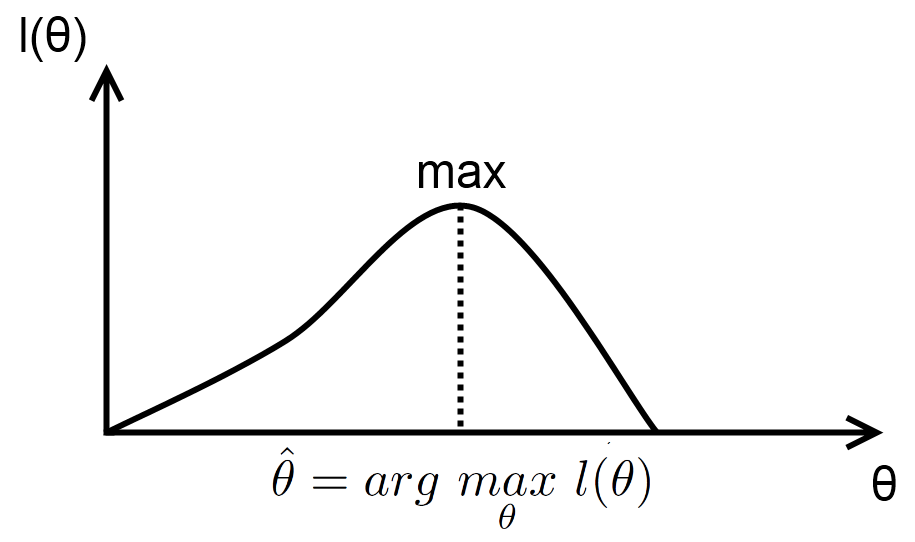
\includegraphics[width=7cm]{./images/MaxLikely.png}
  \end{minipage}
  
  The solution can be the true global maximum, a local maximum or minimum. Also check the boundaries of the parameter space for a possible maximum.
  \skriptsubsubsection{Gaussian case}{88}
  $\boldsymbol{\hat{\mu}} = \frac1n \sum\limits_{k=1}^n \mathbf{x}_k$ (called sample mean)\\
  $\boldsymbol{\hat{\Sigma}} = \frac1n \sum\limits_{k=1}^n 
  (\boldsymbol{x}_k - \boldsymbol{\hat{\mu}})(\boldsymbol{x}_k - \boldsymbol{\hat{\mu}})^T$ (called sample covariance)
  
  \skriptsubsubsection{Bias}{89}
  An estimation is biased if $E(\boldsymbol{\hat{\theta}}) \neq \theta$ or in words: if the expected 
  value of an estimation is not equal to the true value.
  E.g. the variance of a Gaussian distribution is biased.\\
  \subsubsubsection{Unbiased Estimator} of the variance is $\boldsymbol{C} = \frac1{n-1} \sum\limits_{k=1}^n 
  (\boldsymbol{x}_k - \boldsymbol{\hat{\mu}})(\boldsymbol{x}_k - \boldsymbol{\hat{\mu}})^T$ called sample covariance matrix.
  
  
  \skriptsubsection{Bayesian Estimation}{90}
  In Bayesian learning, we consider $\boldsymbol{\theta}$ to be a random variable and estimate the distribution of this variable.
  The main difference to the maximum-likelihood method is that we give to our guess for the $\boldsymbol{\hat{\mu}}$ and $\boldsymbol{\hat{\Sigma}}$ an 
   uncertainty\slash{}variance\slash{}distribution. Additionally the Bayes method can use prior knowledge. If there is such a prior knowledge Bayesian is possible 
   to reach the same result as ML with less training data. A disadvantage is, that it needs more calculating power, or better result with same training data, if the class-conditional density is known.
  
  \skriptsubsubsection{Class-Conditional Densities}{91}
  The heart of Bayesian classification: Computation of posterior probabilities. This is the 
  general formula:
  $$P(\omega_i|\bm{x}, \mathcal{D}) = \frac{p(\bm{x}|\omega_i, \mathcal{D}) P(\omega_i|\mathcal{D})}
    {\sum\limits_{j=1}^{c} p(\bm{x}|\omega_j, \mathcal{D}) P(\omega_j|\mathcal{D})}$$
    
    
  The assumption is that the prior probabilities are known or obtainable from a trivial calculation $P(\omega_i|\mathcal{D})=P(\omega_i)$.
  Furthermore, the training samples $\mathcal{D}_i$ now belong to categories $\omega_i$, 
  ($i=1,\ldots,c$) and the samples of category $i$ are not influenced by category $j$ ($j \neq i$).
  Now, each category can be treated indepently.
  $$P(\omega_i|\bm{x}, \mathcal{D}) = \frac{p(\bm{x}|\omega_i, \mathcal{D}_i) P(\omega_i)}
    {\sum\limits_{j=1}^{c} p(\bm{x}|\omega_j, \mathcal{D}_j) P(\omega_j)}$$
    
  \skriptsubsubsection{Parameter Distribution}{91}
  We want to find the distribution of a parameter vector $\bm{\theta}$ for every class with a given dataset $\mathcal{D}$:
  $$\underbrace{p(\bm x |\omega_i)}_{\text{Likelihood}}\approx \underbrace{p(\bm{x}|\mathcal{D},\omega_i)}_{\text{Posterior}} = \int{p(\bm{x,\theta}|\mathcal{D}) d \bm{\theta}}\overset{!*}{=}
  \underbrace{\int}_{\text{
  	\parbox{2.3cm}{\centering 
  		Multidimensional, hard to compute}}  
	}
  \underbrace{p(\bm{x}|\bm{\theta})}_{\text{Model}} 
  \underbrace{p(\bm{\theta}|\mathcal{D})}_{\text{given by training data}} d\bm{\theta}$$
 *: Because the selection of $\bm{x}$ and that of $\mathcal{D}$ is done independently.
  \skriptsubsubsection{Gaussian case: Univariate case}{92}
  with known $\sigma=\Sigma$. e.g. known measurement system but unknown measurement value\\
  \subsubsubsection{Finding the A Posteriori Density}
  \begin{aufzaehlung}
    \item Model: $p(x|\mu) \sim N(\mu, \sigma^2)$ ($\sigma^2$ is known)
    \item Goal: Finding $\mu$ as the only unknown parameter
    \item Best prior guess: $p(\mu) \sim N(\mu_0, \sigma_0^2)$
    \item Crucial assumption: Knowing the prior distribution of $\mu$ ($\mu$ is normal distributed).
    \item The Bayes formula is introduced: 
      $p(\mu|\mathcal{D}) = \frac{p(\mathcal{D}|\mu) p(\mu)}{\int p(\mathcal{D}|\mu) p(\mu) d\mu} = \frac{p(\mathcal{D}|\mu) p(\mu)}{p(\mathcal{D})}$
    \item And by forward calculation: 
      $p(\mu|\mathcal{D}) = \frac{1}{\sqrt{2\pi} \sigma_n} \exp[-\frac12 (\frac{\mu-\mu_n}{\sigma_n})^2]$
      with $n$ as the number of samples (which can be increased). 
      $p(\mu|\mathcal{D})$ is called \em reproducing density \em and $p(\mu)$ is a \em conjugate prior \em.
    \item After some calculation, this results in
      $$\mu_n = (\frac{n\sigma_0^2}{n\sigma_0^2 + \sigma^2})\hat{\mu}_n + 
      \frac{\sigma^2}{n\sigma_0^2 + \sigma^2} \mu_0 \quad \text{ with } \quad
      \hat{\mu}_n = \frac1n \sum\limits_{k=1}^{n}x_k. \text{ (Sample Mean)}$$
      At the beginning ($n=0$), the initial value is weighted high ($\mu_0$) but with more samples
      the sample mean is weighted much higher ($\hat{\mu}_n$) and the initial knowledge is getting 
      unimportant when $n \rightarrow \infty$.\\
      The variance of the parameter distribution is
      $$\sigma_n^2 = \frac{\sigma_0^2 \sigma^2}{n\sigma_0^2 + \sigma^2}$$
      which leads to a Dirac delta function when $n \rightarrow \infty$.
  \end{aufzaehlung}
  
  \subsubsubsection{Finding the Class-Conditional Density}
  $$p(x|\mathcal{D}) = \int p(x|\mu) p(\mu|\mathcal{D}) d\mu \sim N(\mu_n, \sigma^2+\sigma_n^2)$$ 
    
  \skriptsubsubsection{Gaussian case: Multivariate case}{95}
  with known $\bm\Sigma$ but unknown $\bm{\mu}$.\\
  The generalization of the a posteriori calculation leads to:
  $$\bm{\mu}_n = \bm{\Sigma}_0 \Big(\bm{\Sigma}_0 + \frac1n \bm{\Sigma}\Big)^{-1}\bm{\hat{\mu}}_n +
    \frac1n \bm{\Sigma} \Big(\bm{\Sigma}_0 + \frac1n \bm{\Sigma}\Big)^{-1} \bm{\mu}_0,$$
  its variance
  $$\bm{\Sigma}_n = \bm{\Sigma}_0 \Big( \bm{\Sigma}_0 + 
    \frac1n \bm{\Sigma}\Big)^{-1}\; \frac1n{\bm{\Sigma}}$$
  
  and the class-conditional density is
  $$p(\bm{x}|\mathcal{D}) \sim N(\bm{\mu}_n, \bm{\Sigma} + \bm{\Sigma}_n)$$
  
  \skriptsubsubsection{Recursive Bayes Learning}{98}
  \em Bayesian learning \em can be done when the class-conditional density function is expressed 
  as recursive formula and it converges to a Dirac delta function:
  $$p(\bm{\theta} | \mathcal{D}^n) = \frac{p(\bm{x}_n|\bm{\theta}) p(\bm{\theta}| \mathcal{D}^{n-1})}
  {\int p(\bm{x}_n|\bm{\theta}) p(\bm{\theta}|\mathcal{D}^{n-1}) d\bm{\theta}}$$
  
  
  \skriptsubsection{Differences between Bayes and Maximum-Likelihood}{100}
  \begin{tabular}{ll}
    \parbox{9cm}{
      \textbf{Maximum-Likelihood}
      \begin{itemize}
        \item Easier to understand and interpret
        \item Easier to calculate (computational complexity)
        \item Converges to Bayes solution with infinite data
      \end{itemize}
    }
    & \parbox{9cm}{
      \textbf{Bayesian Estimation}
      \begin{itemize}
        \item Requires prior knowledge (or assumptions)
        \item Can reach better results with less training data
        \item Converges to ML solution with infinite data
      \end{itemize}
    }
  \end{tabular}
  
  Some sources of classification errors do both have in common:
  \begin{itemize}
    \item \textbf{Bayes or indistinguishability error}: No elimination possible due to overlapping
    densities $p(\bm{x}|\omega_i)$
  	\item \textbf{Model error}: Having an incorrect model leads to wrong results.
  	\item \textbf{Estimation error}: Having a limited number of samples (increasing training data can help reducing)
  \end{itemize}
  
  
  \skriptsubsection{Problems of Dimensionality}{107}
  Many dimensions lead to computational complexity but the classification accuracy might be better.
  
  \skriptsubsubsection{Different Distributions (Accuracy, Dimension, Training Sample Size)}{107}
  Table on p.108/109
  \skriptsubsubsection{Computational Complexity}{111}
  Notion for computational complexity: Said: ``$f(x)$ is of the order of $h(x)$'' and denote this as
  $f(x) = O(h(x))$ (``Big Oh''). E.g. for $f(x) = a_0+a_1x+a_2x^2$ we have: $f(x) = O(x^2)$.
  This Big Oh can be calculated for time or space and is independent of the actual operation but
  only on its scaling. \\
  
  Finding the sample mean $\hat{\boldsymbol{\mu}}$ for $d$ dimensions and $n$ samples is $O(nd)$.
  The complexity of the covariance matrix $\hat{\boldsymbol{\Sigma}}$ is $O(d^2n)$. 
  The inverse and the determinant each have a complexity of $O(d^3)$.
  
  \subsection{Component Analysis and Discriminants}
  
  \begin{minipage}{13cm}
  
  \skriptsubsubsection{Principal Component Analysis (PCA)}{115}
  Ideal for compression but not for pattern recognition.
  Although PCA finds components that are useful for representing data, there is no reason to 
  assume that these components must be useful for discriminating between data in different classes.\\
  \begin{align*}
	&  && \bm{x}=\bm{m}+a \bm{e} \quad \Rightarrow \quad a_k=\bm{e}^T(\bm{x}_k-\bm{m}) \\
    &\text{Scatter matrix} \quad && \bm{S} = \sum\limits_{k=1}^{n}{(\bm{x}_k-\bm{m})(\bm{x}_k-\bm{m})^T} \\
    &\text{Eigenvector } \bm{e} \quad && \bm{S e}=\lambda \bm{e} \\
    &\text{Results in} && \bm{x}=\bm{m}+\sum\limits_{i=1}^{d'}{a_i \bm{e}_i}
  \end{align*}

  \end{minipage}
  \begin{minipage}{5cm}
  	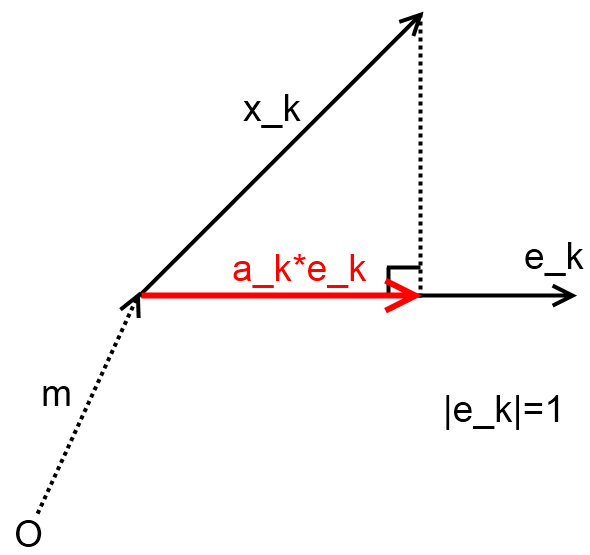
\includegraphics[width=5cm]{./images/principalComp.png}
  \end{minipage} 
  
  \skriptsubsubsection{Fisher Linear Discriminant}{117}
  \begin{minipage}{10.5cm}
  Very cool (according to Guido).
    \begin{aufzaehlung}
      \item Calculate the $d$-dimensional sample mean for every class
        $\bm{m}_i = \frac{1}{n_i} \sum\limits_{\bm{x} \in \mathcal{D}_i} \bm{x}$
      \item Obtain scatter matrices (= covariance matrix without division of N):
        $\bm{S}_i = \sum\limits_{\bm{x} \in \mathcal{D}_i} 
        (\bm{x}-\bm{m}_i) (\bm{x}-\bm{m}_i)^T$
        and the within-class scatter matrix for the two-category case
        $\bm{S}_W = \bm{S}_1 + \bm{S}_2$
      \item Finding the Fisher linear discriminant:
        $\bm{w} = \bm{S}_W^{-1} (\bm{m}_1 - \bm{m}_2)$
        (normalize to$||\bm{w}||=1$.)
      \item Now we can transform and reduce dimensionality to a scalar:
        $y = \bm{w}^T \bm{x}$
    \end{aufzaehlung}
  \end{minipage}\hspace{5mm}
  \begin{minipage}{8cm}
    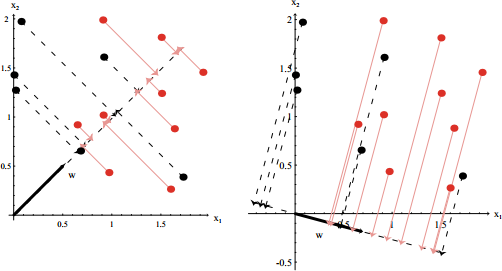
\includegraphics[width=8cm]{./images/fisher_discriminant.png}
  \end{minipage}
  
  \skriptsubsection{Hidden Markov Models}{128}
  \begin{minipage}{11cm}
    Hidden Markov Models (HMMs) are used to model timing dependencies, e.g.  
    in speech recognition the order of the characters.
    
    Problems:
    \begin{liste}
      \item Evaluation problem: Determine the \em probability \em that a particular sequence of 
      visible states $\bm V_T$ was generated by \em that model\em.
      \item Decoding problem: Determine the \em most likely sequence of hidden states \em $\bm \omega^T$ that
      led to observations $\bm V_T$.
      \item Learning problem: Given the structure and training observations, \em learn the parameters \em
      $a_{ij}$ and $b_{jk}$. 
    \end{liste}
    
    \skriptsubsubsection{Evaluation}{131}
      The Forward algorithm leads to $P(\bm V_T)$ and $\alpha_j(t)$. $\alpha_j(t)$ is the
      probability that the model is in state $\omega_i$ and has generated the target sequence up to step $t$.\\
      
      The Backward algorithm leads to $P(\bm V_T)$ and $\beta_j(t)$. $\beta_j(t)$ is the
      probability that the model is in state $\omega_j$ and the target sequence will be generated from step $t+1$ to the end $T$.
      
      
    \skriptsubsubsection{Decoding}{135}
      The Decoding algorithm from the book can return impossible solutions due to the fact that
      the $a_{ij}$ are not considered completely. Use the Viterbi decoder instead.
    
    \skriptsubsubsection{Learning}{137}
      The Forward-Backward (Baum-Welch) algorithm is an iterative algorithm which finds the HMM 
      weights $a_{ij}$ and $b_{ik}$ in a local optimum.
      \begin{aufzaehlung}
        \item Initialize $a_{ij}$, $b_{ik}$ with prior knowledge or uniformly distributed
        \item Loop start
        \item Use the Forward and Backward algorithms to find out $\alpha_i(t)$, $\beta_j(t)$ and $P(\bm V_T|\bm \Theta)$
        \item Calculate $\gamma_{ij}(t)$, $a_{ij} = \hat a_{ij}$, $b_{jk} = \hat b_{jk}$
        \item Restart loop when $a_{ij}$ and $b_{jk}$ didn't change a lot ($\delta_1$) or 
        $P(\bm V_T|\bm \Theta)$ didn't change a lot ($\delta_2$)
      \end{aufzaehlung}
      
  \end{minipage}\hspace{5mm}
  \begin{minipage}{8cm}
	\hspace{1cm}
    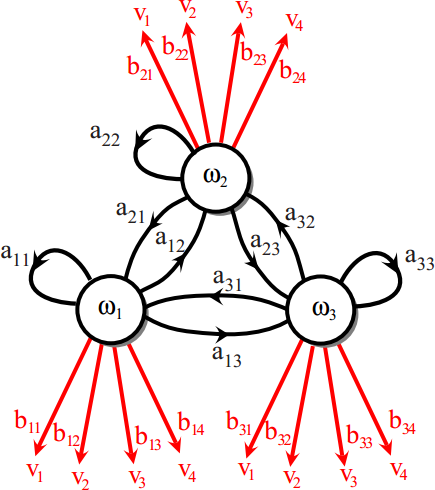
\includegraphics[width=5cm]{./images/hiddenMarkovModel.png}
    
    \begin{tabular}{ll}
      Hidden states              &$\omega_i$\\
      Absorbing/final state      &$\omega(T) = \omega_0$\\
      Visible states             &$\bm V_T = [v_1, \ldots, v_T]$\\
      Transition probability     &$a_{ij} = P(\omega_j(t+1) | \omega_i(t))$\\
      Emission probability       &$b_{jk} = P(v_k(t) | \omega_j(t))$\\
      $\sum\limits_j a_{ij} = 1$ &$\sum\limits_k b_{jk} = 1$\\
    \end{tabular}
    
    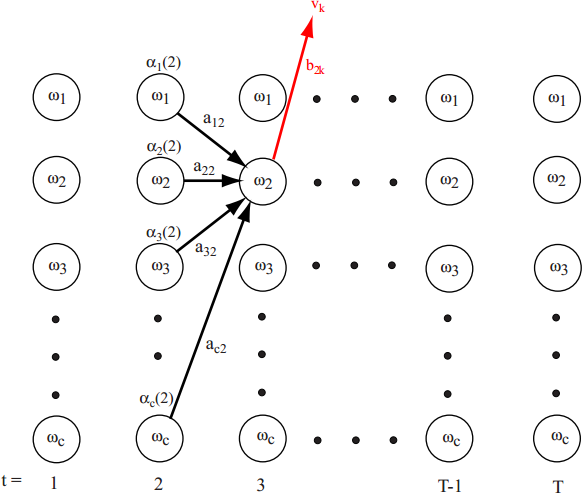
\includegraphics[width=7cm]{./images/hiddenMarkovModel2.png}
  \end{minipage}
  

\skriptsection{Nonparametric Techniques}{161}
  The assumption, that the forms of the underlying density functions are known is not the case in 
  most pattern classification problems.
  
  
  When $V$ is the volume of a region $\mathcal{R}$, the number of samples which fall into this
  region can be counted and the probability of a sample falling into this region can be 
  approximated:
  $$p(\bm{x}) \approx \frac{k/n}{V}$$
  where $k$ is the number of samples that fall in $\mathcal{R}$ and $n$ is the total number of training
  samples (of this class). Therefore, $k/n$ is the relative frequency.
  
  Two approaches solve these problems:\\
  \begin{center}
    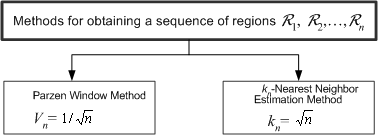
\includegraphics[width=7cm]{./images/non-parametric_methods_1.png}\hspace{0.5cm}
    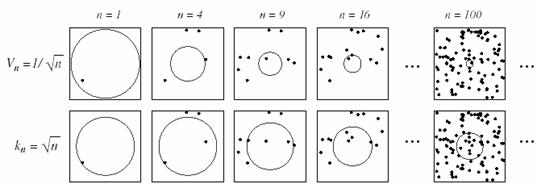
\includegraphics[width=7cm]{./images/non-parametric_methods_2.jpg}
  \end{center}
    
  \skriptsubsection{Parzen Windows}{164}
  	The goal of the Parzen Windows method is to estimate a class-conditional probabilty density function $p(\bm x | \omega)$. 
    For this a window function with a defined region $\mathcal{R}_n$ is convoluted with each training sample of a given class. 
    The sum of all functions gives the density function.\\
    The window function could be, for example, a $d$-dimensional hypercube with $h_n$ being the length of an edge or any other function 
    (Gauss, triangle (Dreieck), \ldots). 
    Often a window with infinite length such as the Gauss window is used, because then the probability will never be zero and a better comparison can be made.\\
    \begin{minipage}{13cm}
    	$$\varphi_{\mathrm{hypercube}}(\bm{u}) = \begin{cases}
	    1 &|u_j| \leq 1/2 \quad  j=1,\ldots,d\\
	    0 & \text{otherwise}
	    \end{cases}$$
	    Therefore, the probability can be estimated with
	    $$p(\bm{x}|\omega_j) = \frac1{n_j} \sum_{i=1}^{n_j} \frac{1}{V_{n_j}} \varphi \left(\frac{\bm{x}-\bm{x}_i}{h_{n_j}} \right) \quad 
	    \text{with } \varphi(\bm{x}) \geq 0 \text{ and } \int \varphi(\bm{u}) du = 1 $$
	    $n_j$ is the number of training sample given class $j$. \\
    \end{minipage}
    \begin{minipage}{5cm}
        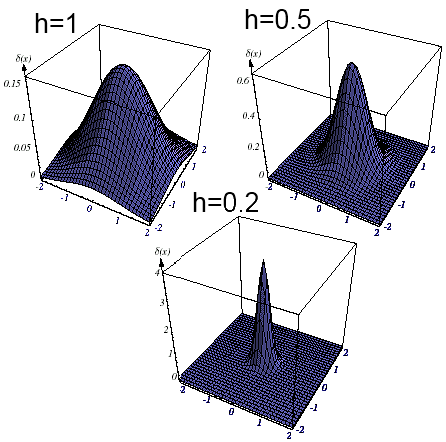
\includegraphics[width=4cm]{./images/parzenWindow.png}
    \end{minipage}
    
    Choosing $h_n$ is important! If $h_n$ (which leads to $V_n$) is too large, the resolution of the
    estimate is too small; if $h_n$ is too small, the statistical variability is too high.
    
    If we define $\delta_n(\bfx)$ to be $\delta_n(\bfx) = \frac{1}{V_n} \varphi\left(\frac{\bfx}{h_n}\right)$,
    we can rewrite $p_n(\bfx)$ as the average of a number of dirac functions 
    \begin{equation*}
      p_n(\bfx) = \frac{1}{n}\sum\limits_{i=1}^{n}\delta_n(\bfx-\bfx_i)
    \end{equation*}
   
  
  \skriptsubsubsection{Probabilistic Neural Networks}{172}
  A PNN is a Parzen window with a Gaussian window function where all data has to be normalized.\\
    \begin{tabular}{ll}
      \parbox{7cm}{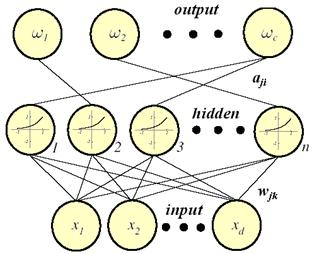
\includegraphics[width=5.5cm]{./images/probabilistic_neural_network.jpg}}
      & \parbox{11cm}{
      Legend:
      \begin{liste}
        \item $d$ input units
        \item $n$ pattern units (one per training sample)
        \item $d$ dimensions
        \item $c$ categories ($\omega_i, i=1,\ldots,c$)
        \item Connections from input to pattern units are modifiable weights, which are trained.
        Now $\bm{w}$ is used instead of $\bm{\theta}$.
        \item \hilight{All (training and input) data must be normalized}: $\sum\limits_{i=1}^d x_i^2 = 1$
      \end{liste}}
    \end{tabular}
    
    \subsubsubsection{Training} is quite easy. Add a new hidden node, set $\bm{w}_k = \frac{\bm{x}_k}{\sqrt{||x||^2}}$ for all training samples 
    and connect every node to the specific category $\omega_k$.
    
    \subsubsubsection{Classification} uses an activation function 
    $\varphi\Big(\frac{\bm{x}-\bm{w}_k}{h_n}\Big) = e^{\frac{\bm{w}_k^T \bm{x}-1}{\sigma^2}}$ 
    with $\sigma$ being a degree of freedom.
    
    PNNs have a high learning speed but need a lot of memory (high space complexity). However,
    speed complexity can be reduced easily by implementing the net activation function evaluation in
    parallel.
    
  
  \skriptsubsection{$k_n$-Nearest-Neighbor Estimation}{174}%TODO: continue
    \begin{tabular}{ll}
      \parbox{7cm}{
        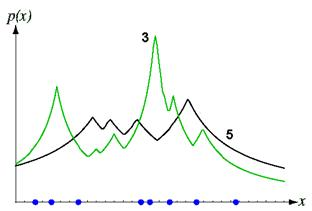
\includegraphics[width=6cm]{./images/k-nearest-neighbor.jpg}
          }
        & \parbox{11cm}{
          Instead of searching the best window function, it can also be adjusted to the training data 
          (also called \em prototypes\em).
          
          Regarding the probability function $p_n(\bm{x}) = \frac{k_n/n}{V_n}$, $k_n$ and $n$
          and therefore $k_n/n$ are fixed and only the volume is adjusted. $k_n$ is now the degree 
          of freedom and a good value can be $k_n = \sqrt{n}$.
          
          The figure shows the training samples on the $x$-axis and two possible probabilities
          with $k_n=3$ and $k_n=5$. The curve is continuous, but the first derivation (slope) is not. 
          The $k_n$-Nearest-Neighbor curve is spikier in comparison to the Parzen-Window estimation, especially when a Gaussian window is used 
          in the Parzen window method.
          }
    \end{tabular} 
    \vspace{3mm}\\
    Instead of estimating the probability density and calculate the \textbf{a posteriori probabilities} $\bm {P(\omega_i | \bm x)}$ with Bayes, the a posteriori 
    probabilities can be directly calculated out of the training data:\\
    $$ P_n(\omega_i|\bm x)=\frac{k_i}{k}$$
    where $k_i$ is the number of training sample of class $\omega_i$ within a volume $V$ around $\bm x$.
    $k$ is the total number of training samples also within the volume $V$.
  
  
  \skriptsubsection{Nearest-Neighbor Rule}{177}
  	The nearest-neighbor is a simplification of $k_n$-nearest-neighbors, in particular $k=1$. 
  	The given test sample will be the same class as the ``next'' training sample.
  	This can be visualized by a \emph{Voronoi tesselation}\formelbuch{178}.
  	
  	\skriptsubsubsection{Convergence of the Nearest Neighbor}{179}
    The error rate of the nearest-neighbor rule is not optimal, it is usually worse than the Bayes 
    rate (minimum). However, it is never worse than twice the Bayes rate. 
    In the best case, if the a-posteriori probabilities of all classes are the same
    the error rate is the same as the Bayes error rate ($\frac{c-1}{c}$).\qquad Error bound: $P^*\leq P\leq P^*\left(2-\frac{c}{c-1}P^*\right)\approx 2P^*$ \\

  \begin{minipage}{14.5cm}
		\skriptsubsection{$k$-Nearest-Neighbor Rule}{182}
		The classifier assigns the label $\omega_m$ to the input of the highest number of samples among the $k$
		nearest samples. Therefore, $k$ shouldn't be a multiple of the number of classes $c$. 
		The error rate is better than with Nearest-Neighbor. If $k=\infty$
		the error rate will be the same as the Bayes error rate. 
		
		This can also be seen as an estimate of the a posteriori probabilities $P(\omega_i|\bm x)$.
		
		\skriptsubsection{Computational Complexity}{184}
  \end{minipage}
  \hfill
  \begin{minipage}{4cm}
	  	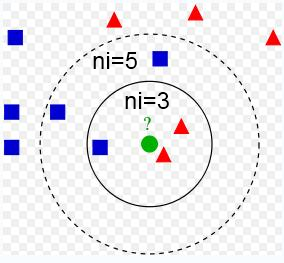
\includegraphics[width=4cm]{./images/kNearest.png}
  \end{minipage}
  
    High complexity in space and time especially when having a lot of features (dimensionality)!
    Reduce by: 
    \begin{aufzaehlung}
    	\item Use the squared distance instead of the square-root to compare: $D_r(\bm{a},\bm{b})=\sum\limits_{k=1}^r(a_k-b_k)^2$ 
    	instead of  $D_r(\bm{a},\bm{b})=\left(\sum\limits_{k=1}^r(a_k-b_k)^2\right)^{1/2}$
    	\item Calculate partial distances during classification (abort calculating the distance if it 
    	is already higher than the $k$-nearest ones)
    	\item Eliminate unused prototypes (pruning) by algorithm 3\formelbuch{186}. This has the disadvantage that a new training sample can't be easily added.
    	\item Form a search tree during training: Divide search field into subfields (e.g. 2D: 
    	1 search field leads to 4 quadrants). It's much faster, but does not necessarily yield to the best solution.
    \end{aufzaehlung}
  
  \skriptsubsection{Metrics}{187}
    A metric gives a generalized scalar distance between different arguments (vectors, functions, etc.). 
    The metrics have a big influence on the Nearest-Neighbor. \textbf{Scaling!!!}
    Usually all lengths are measured in terms of their standard deviation.
  
  \begin{multicols}{2}

    
    \subsubsection{Properties}
    \begin{tabular}{ll}
      Nonnegativity: &$D(\bm a, \bm b) \geq 0$  \\
      Reflexivity:   &$D(\bm a, \bm b) = 0 \text{ if } \bm a = \bm b$\\
      Symmetry:      &$D(\bm a, \bm b)=D(\bm b, \bm a)$  \\
      Triangle inequality: & $D(\bm a, \bm b) + D(\bm b, \bm c) \geq D(\bm a, \bm c)$
    \end{tabular}
    
    \subsubsection{Euclidean Distance / L2-Norm / Pythagoras}
      Definition: $D(\bm a, \bm b) = \sqrt{\sum\limits_{k=1}^d (a_k - b_k)^2}$
      
      Problem of Euclidean distance (``Pythagoras''): When scaling the axes, the metric changes (e.g. 
      axis $x_1$ is measured in $mm$ and axis $x_2$ in $cm$, the distance is not consistent).
      
      
    \subsubsection{Manhattan Metric / L1-Norm / City Block Distance}
      Shortest path between $\bm a$ and $\bm b$ following the coordinate axis.
    
    \subsubsection{Minkowski Metric / Lk-Norm}
	A general class of metrix for d-dimensional patterns is the $L_k$ norm
	$L_k(\mathbf{a},\mathbf{b}) = \left(\sum\limits_{i=1}^{d} \left| a_i-b_i \right|^k \right)^{1/k}$
    
    \subsubsection{Tanimoto Metric}
	The Tanimoto metric is used in taxonomy to define the distance between two sets.
	$D_{\mathrm{Tanimoto}}(\mathcal{S}_1,\mathcal{S}_2) = \frac{n_1 + n_2 - 2 n_{12}}{n_1 + n_2 - n_{12}}$
	where $n_1$ and $n_2$ are the number of elements in the sets $\mathcal{S}_1$ and $\mathcal{S}_2$ 
	and $n_{12}$ is the number of elements that are in both sets.
    
    \subsubsection{Selection of a Metric}
      Hard to choose, usually selection is dictated by computational concerns not by prior knowledge
      about the distributions.
      
    \skriptsubsubsection{Tangent distance}{188}
      
  \end{multicols}
\skriptsection{Linear Discriminant Functions}{215}
  Assume, that the \emph{form} of the discriminant functions are known instead of the
  distributions. The problem of finding a linear discriminant function can be formulated as a problem
  of \emph{minimizing a criterion function}, e.g. the sample risk or the training error.
  But a small training error doesn't guarantee a small test error.
  

  \skriptsubsection{Linear Discriminant Functions and Decision Surfaces}{216}
    \skriptsubsubsection{Two-Category Case}{216}
      The same forms as in \ref{sec:bayes_discriminant_function} (page \pageref{sec:bayes_discriminant_function}) 
      of this summary are used here:
      $$g(\bm x) = \bm w ^T \bm x + w_0$$
      Decide $\omega_1$ when $g(\bm x) > 0$ and $\omega_2$ when $g(\bm x) < 0$. $g(\bm x) = 0$ is
      the decision surface, it is a hyperplane in the linear case and it is normal to the weights 
      $\bm w$.
      
    \begin{multicols}{2}
	    \skriptsubsubsection{Multicategory Case}{218}
		There exist several possibility to create multicategory classifier with $c$ classes.
		We could use $c$ linear discriminant functions to separate points belonging 
		to $\omega_i$ and those not belonging to $\omega_i$.
		Another possibility would be to create $c(c-1)/2$ discriminants, one for each pair of classes.
		Both aproaches lead to undefined ambiguous regions.
	
		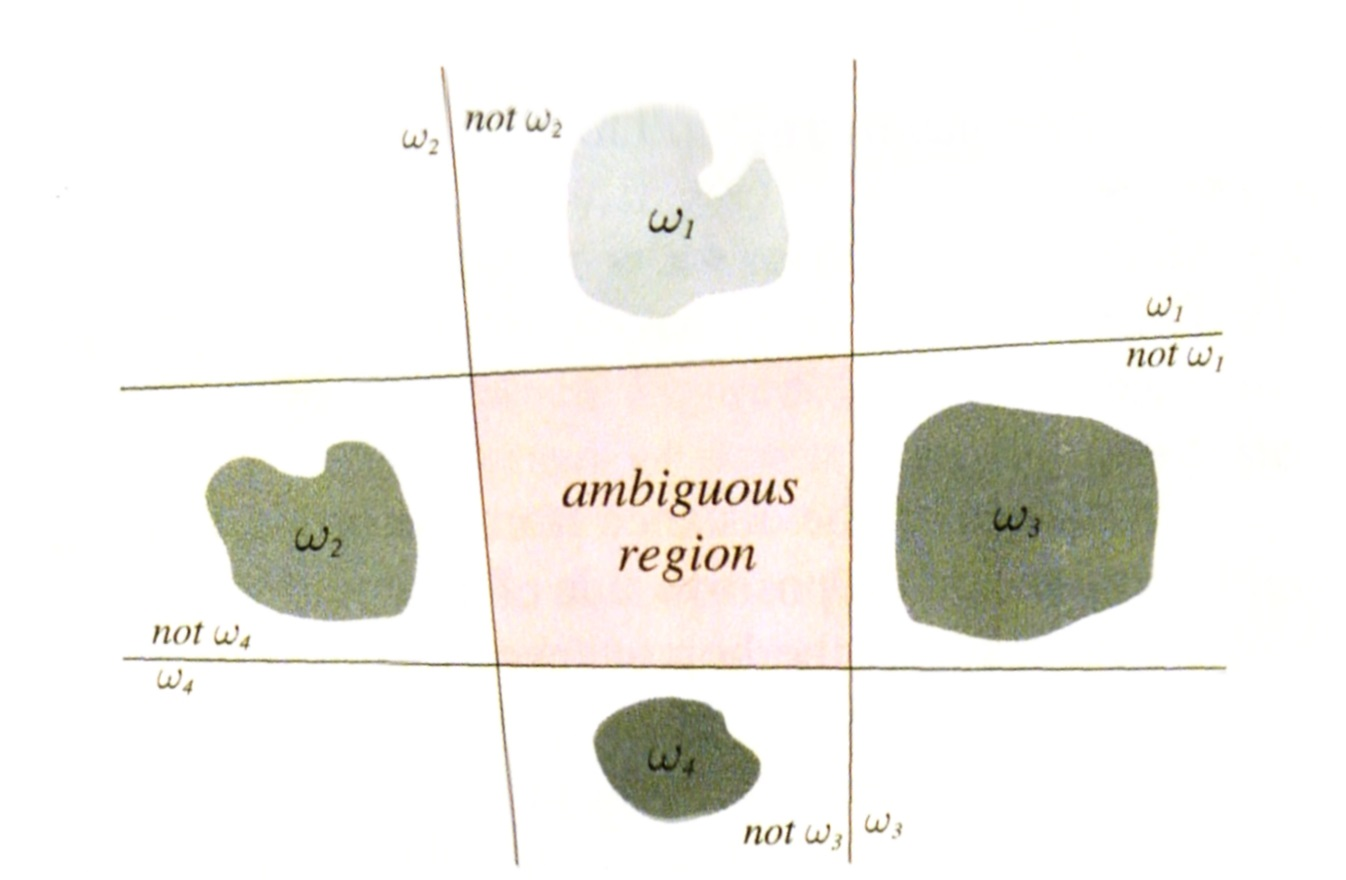
\includegraphics[width=0.5\linewidth]{images/onevsall.jpg}
		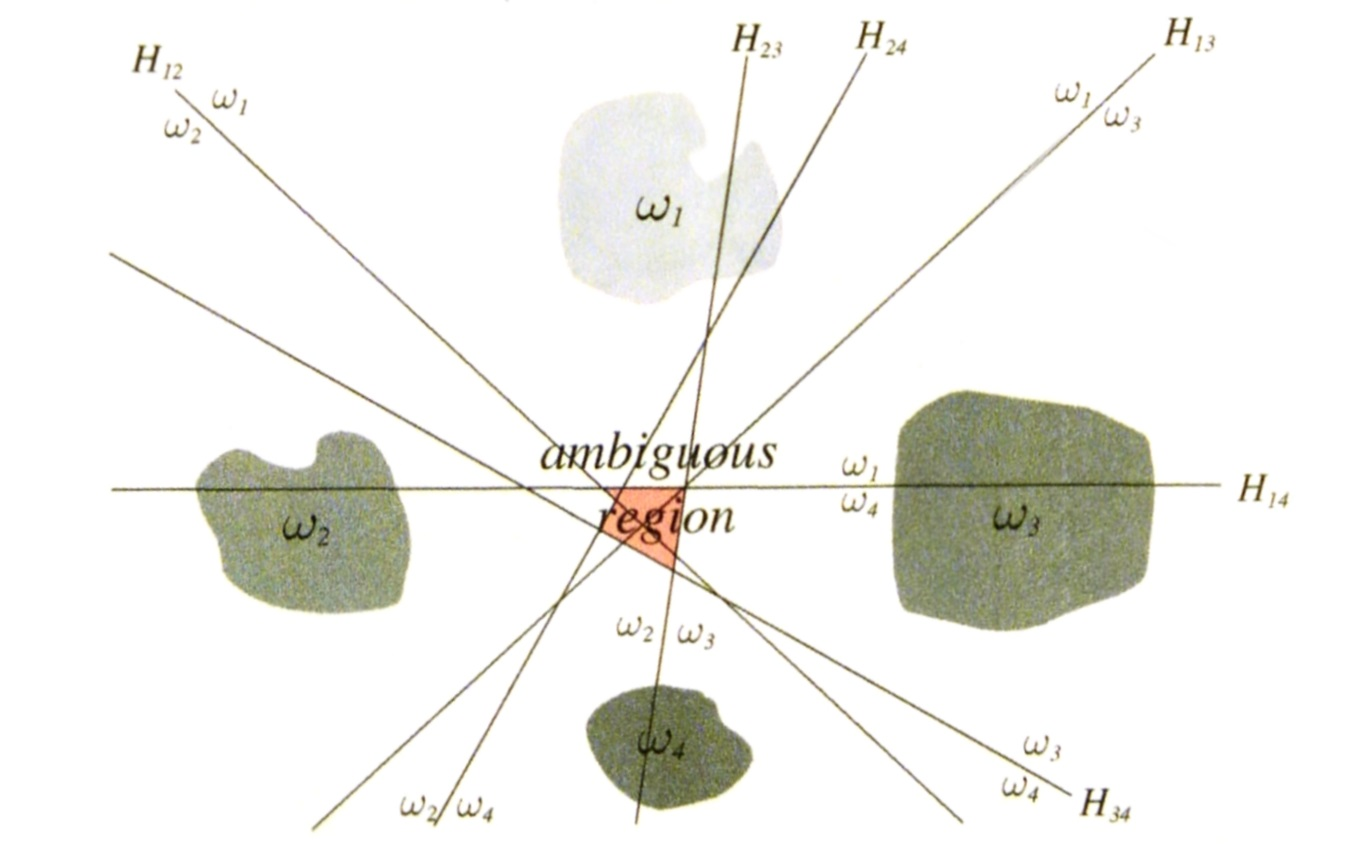
\includegraphics[width=0.5\linewidth]{images/onevsone.jpg}
    \end{multicols}
    
    By defining $c$ linear discriminant functions
    \begin{equation*}
	    g_i(\bfx) = \mathbf{w}_i^t\bfx + w_{i0} \quad i=1,\ldots,c
    \end{equation*}
	we can assign $\bfx$ to $\omega_i$ if $g_i(\bfx) > g_j(\bfx)$ for all $j \neq i$.
	This classifier is called a \emph{linear machine}.
      
  
  \skriptsubsection{Generalized Linear Discriminant Functions}{219}
  \label{sec:generalized_linear_discriminant_function}
  
  \begin{multicols}{2}
	  \subsubsection{Quadratic Discriminant Function}
	      By multiplying features with itself, ``new'' features can be created and possibly improve the classification
	      results. This results in the quadratic discriminant function
	      
	      \begin{equation*}
		      g(\bm x) = w_0 + \sum\limits_{i=1}^d w_i x_i + \sum\limits_{i=1}^d \sum\limits_{i=1}^d w_{ij} \underbrace{x_i x_j}_{\text{new feature}}
	      \end{equation*}
	      
	      and can produce more complicated separating surfaces, because the problem will be mapped in a more dimensional space.
	      The data itself uses not more dimensions. E.g. The data of an one dimension problem stays on one line. \\
	      
      	 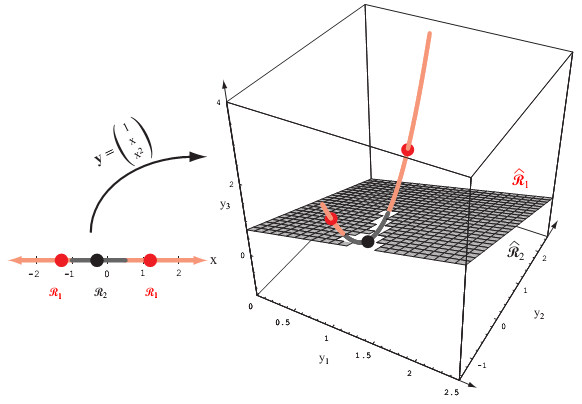
\includegraphics[width=6cm]{./images/map1DTo2D.png} \\
       	 Feature mapping from one dimension into 2D with $x^2$ \\
       \columnbreak	 
   	   \subsubsection{Generalized Linear Discriminant Functions}
   	     By continuing this approach, polynomial discriminant function or generalized linear discriminant 
   	     functions are evolving: 
   	     $$g(\bm x) = \sum\limits_{i=1}^{\hat d} a_i y_i(\bm x) = \bm a^T \bm y$$
   	     $\bm a$ is a 
   	     $\hat d$-dimensional weight vector and the $\hat d$ functions $y_i(\bm x)$ ($\varphi$-functions 
   	     or augmented features) are arbitrary functions of $\bm x$ and \textbf{don't have to be linear}.
   	     Therefore, the discriminant functions are linear in $\bm y$ but not in $\bm x$.\\
   	     The disadvantage is a high computational complexity with high dimensions and that much 
   	     \textbf{more trainings data} are needed to avoid overfitting.
   	     
    \subsubsection{Augmented Feature Vector}
      To include the offset $w_0$ of the discriminant function $g(\bm x) = w_0 + w_1 x_1 + w_2 x_2 + \ldots + w_n x_d$ into the weight vector $\bm w$ 
      a one is added to the feature vector  $\bm y = [1, x_1, x_2, \ldots, x_n]^T = [1, \bm x]^T$.
      This vector is called \emph{augmented feature vector} and the resulting weight vector $\bm a = [w_0, w_1, w_2, \ldots w_d]^T = [w_0, \bm w]^T$  \emph{augmented
      weight vector}.
      The discriminant function can then be written as $g(x) = \mathbf{a}^T \mathbf{y}$.
      The decision boundary can now be interpreted as a hyperplane going through $[0,\ldots,0]$ and 
      all data lies on the level at $y_0=1$.
      The separation plane equation is then $\mathbf{a}^T \mathbf{y} = 0$ with $\mathbf{y} = \begin{bmatrix}1 & x_1& x_2\end{bmatrix} \Rightarrow x_1=-\frac{a_0 + a_2\cdot x_2}{a_1}$
  \end{multicols}      


   
  \subsection{Two-Category Linearly Separable Case}

    If a linear weight vector exists that classifies all samples correctly, then the samples
    are said to be linearly separable.

    \begin{minipage}{11cm}
    
    \skriptsubsubsection{Normalization / Margin}{223}
    In the separable case, the vector product of every training sample of class $\omega_1$ with the solution
    vector $\bm a$ is positive, and with the class $\omega_2$ is negative.\\
    For easier handling of the training data, all samples labeled $\omega_2$ are replaced by their negatives.
    Now the vector product of the solution vector $\bm a$ with \emph{every} training sample will have to be positive 
    $\bm a^T \bm y_i  > 0$ \\
    
    The separating vector usually doesn't have one single solution but it can lie in a solution
    region. Furthermore, $\bm a$ should not lie on the boundary and therefore a margin $b$
    can be introduced. \\
        
    A normalized augmented feature for a 2-dimensional problem can then look like:
    $\bm y = \begin{bmatrix}
      1 & 1 & 2\\
      1 & 2 & 0\\
      -1 & -3 & -1\\
      -1 & -2 & -3
    \end{bmatrix}$.
    \end{minipage}
    \hspace{5mm}
    \begin{minipage}{7cm}
    	 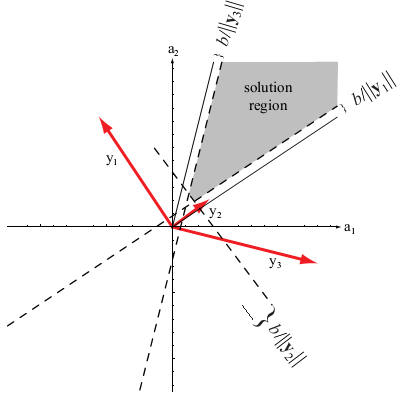
\includegraphics[width=7cm]{./images/solutionRegionWithMargin.png}
    	 Solution region of a ``normalized" vector with margin $b$
 	\end{minipage}
    
    \skriptsubsubsection{Basic Gradient Descent}{224}
      The basic approach to find a solution vector is the method of steepest descent. The aim is to
      minimize a defined criterion function $J_a$ and it is solved iteratively with every step calculating
      $$\bm a (1) \text{ arbitrary}$$
      $$\bm a (k+1) =  \bm a(k) - \eta(k) \nabla J(\bm a(k))$$
      with $\eta > 0$ being the step size or learning rate. When $\eta$ is too small, convergence is
      needlessly slow, with $\eta$ being large the correction can overshoot and even diverge.\\
      The \textbf{optimal step size} can be calculated with:
      $\eta(k)= \frac{\|\bm{\nabla J}\|^2}{\bm{\nabla J^T  H \nabla J}}$ where $\bm H$ is the Hessian matrix
       (matrix of second partial derivatives $\partial^2 J / \partial a_i \partial a_j$, see Newton's Algorithm).
      Calculating the Hessian matrix in every step is normally too expensive so that the optimal solution is used very seldom.

    \skriptsubsubsection{Newton's Algorithm}{226}
      The Newton method is not used widely due to the fact that a matrix has to be inverted on every
      step:
      $$\bm a(k+1) = \bm a(k) - \bm H^{-1} \bm \nabla \bm J \text{ with Hessian matrix } \bm H = \begin{bmatrix}
      \frac{\delta^2 f}{\delta x_1^2} & \ldots & \frac{\delta^2 f}{\delta x_1 \delta x_n}\\
      \vdots & \ddots & \vdots \\
      \frac{\delta^2 f}{\delta x_n \delta x_1} & \ldots & \frac{\delta^2 f}{\delta x_n^2}\\
      \end{bmatrix}$$
      This is a simplification of the optimum step size from the section above.
  
  \skriptsubsubsection{Minimizing the Perceptron Criterion Function}{227}
  \begin{minipage}{12cm}
    The problem is to construct a criterion function for solving the linear inequalities $\bm a^T \bm y > 0$. 
    A criteria function which just counts the misclassified sample would be constant at the most position. 
    Therefore the steepest descent would not work. \\
    
    A better idea is the \textbf{Perceptron Criterion Function}
    $\bm J_p(\bm a) = \sum\limits_{\bm y \in \mathcal{Y}_k} (-\bm a^T \bm y)$  with $\mathcal{Y}$ as the set
    of misclassified samples by the current weight vector $\bm a$.\\
    The gradient is $\bm {\nabla J}_p = \sum\limits_{\bm y\in \mathcal{Y}_k} -\bm y$
    which leads to the update rule 
    \begin{equation*}
        \bm a(k+1) = \bm a(k) + \eta(k) \sum\limits_{\bm y\in \mathcal{Y}_k} \bm y
    \end{equation*}
       
   	\end{minipage}
    \hspace{8mm} 
    \begin{minipage}{6cm}
    	 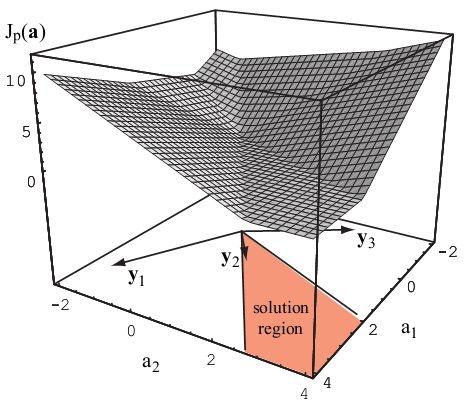
\includegraphics[width=6cm]{./images/perceptron.png}
    \end{minipage} \\
    
    \begin{multicols}{3}
        \skriptsubsubsubsection{Batch Perceptron}{228}\\
        The batch perceptron algorithm yields in a solution for linearly separable problems. 
        It sums up all misclassified samples and then performs a weight update (batch). 
        This has to be done until all of the samples will be classified correctly.  
    \vfill
    \columnbreak
        \skriptsubsubsubsection{Fixed-Increment Single-Sample Perceptron}{230}\\
        The fixed-increment single-sample perceptron algorithm changes the weight vector
        with every (misclassified) sample and therefore saves many computations.
    \vfill
    \columnbreak
        \skriptsubsubsubsection{Variable-Increment Perceptron with Margin}{233}\\
        Additionally, the increment factor $\eta(k)$ can be variable. E.g. $\eta(k)=1/k$. For better 
        generalization, a margin $b$ can be added as shown in algorithm 5.  
    \end{multicols}

    
    \skriptsubsubsection{Relaxation Procedures}{235}
    \begin{minipage}{12cm}
    The \emph{descent algorithm} uses a square in the criterion function:
	$\bm J_q(\bm a) = \sum\limits_{\bm y \in \mathcal{Y}_k} (\bm a^T \bm y)^2$ with $\mathcal{Y}$ as the set
    of misclassified samples.\\
    
  	Because the gradient is continuous, the criterion function $\bm J_q$ is smoother. The problem is that the algorithm is too smooth at the border and 
  	the algorithm can converge to the border or worse to $\bm a=0$. 
  	Another problem is that $\bm J_q$ is dominated by long training samples. \\
  	
  	A criterion function which solves both problems is: 
  	$\bm J_r(\bm a) = \frac{1}{2} \sum\limits_{\bm y \in \mathcal{Y}_k} \frac{(\bm a^T \bm y - b)^2}{\|\bm y\|^2}$
  	where $b$ is a new margin and $\mathcal{Y}(\bm a)$ is the set of samples for which $\bm a^T \bm y \leq b$. $J_r$ is never 
  	negative and only zero when the whole set has been classified correctly inside margin.
  	
  	This leads to the update rule
  	$\mathbf{a}(k+1) = \mathbf{a}(k) + \eta(k)\sum_{\mathbf{y}\in\mathcal{Y}}\frac{b-\mathbf{a}^t\mathbf{y}}{||\mathbf{y}||^2}\mathbf{y}$
  	and the single-sample correction rule
  	$\mathbf{a}(k+1) = \mathbf{a}(k) + \eta \frac{b-\mathbf{a}^t(k)\mathbf{y}^k}{||\mathbf{y}^k||^2}\mathbf{y}^k$
  	where $\mathbf{y}^k$ is the $k$th sample.
	   
    \end{minipage}
    \hspace{8mm}
    \begin{minipage}{6.4cm}
    	 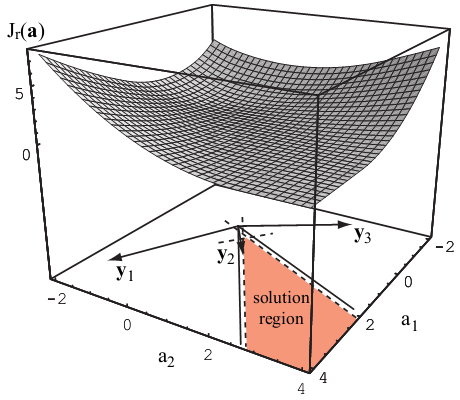
\includegraphics[width=6cm]{./images/relaxation.png}
    	 Criterion function of $\bm J_r(a)$ with margin $b$
    \end{minipage}
    
    \skriptsubsection{Nonseparable Behavior}{238}
    The algorithms up to now won't stop if the data is not separable. Moreover, we do not know if we get a ``good'' result if we stop after a long time.
    One way is to reduce the influence of the wrong classified sample with $\eta(k)=1/k$ so that the solution will end in a ``good'' area.
    
    \skriptsubsection{Minimum Squared-Error Procedures}{240}
    In comparison to the perceptron processes, here all samples are used. 
    The goal is to solve $\bm a^T \bm y_i = b_i$
    \begin{equation*}
    \bm Y \bm a = \bm b
    \qquad \text{or} \qquad
    \begin{bmatrix}
      y_{10} & y_{11} & \ldots & y_{1d}\\
      \vdots &\vdots & & \vdots\\
      \vdots &\vdots & & \vdots\\
      y_{n0} & y_{n1} & \ldots & y_{nd}\\
    \end{bmatrix}
    \begin{array}{c}
    \begin{bmatrix}
    	a_0\\
    	\vdots\\
    	a_d
    \end{bmatrix}\\
    \vphantom{\vdots}\\
    \end{array} = 
    \begin{bmatrix}
    	b_0\\
    	\vdots\\
    	\vdots\\
    	b_n
    \end{bmatrix} \qquad \text{with} \qquad n \gg d
    \end{equation*}
    
    where $\bm{b}$ is the \emph{margin vector} and $b_i$ have to be positive constants. 
    The criterion function $\bm J_S(\bm a)=\|\bm Y \bm a - \bm b \|^2$ lead 
    us to the minimum squared error (MSE) solution of $\bm Y \bm a = \bm b$
    \begin{equation*}
        \bm a = (\bm Y^T \bm Y)^{-1} \bm Y^T b = \bm Y^\dagger \bm b
    \end{equation*}
    where $\bm Y^\dagger \equiv (\bm Y^T \bm Y)^{-1} \bm Y^T$ is the \emph{pseudoinverse} of $\bm Y$.
    If $\bm Y$ is square and nonsingular, the pseudoinverse coincides with the regular inverse. \\

    Disadvantages of these algorithms are: High computational effort for computation of $\bm Y^\dagger$;
    possible singularities ($|\bm Y|$ close to zero); the separating vector is not necessarily found (see next figure);
    no clear abortion criterion (possibly: $|\eta(k) (\bm b - \bm a^T \bm y(k)) \bm y(k)| < \Theta$ with $\Theta$ being a threshold)\\
    
    \begin{wrapfigure}{r}{6cm}
        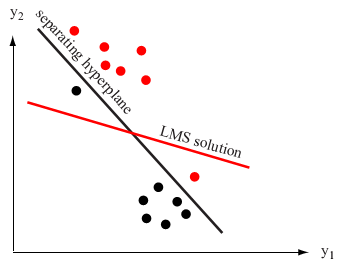
\includegraphics[width=6cm]{./images/LMS.png}
    \end{wrapfigure}
    
     As usual$\bm Y$ is built out of the augmented feature vector of $\omega_1$ and the augmented feature vector of $\omega_2$:\\
    $\bm Y = \begin{bmatrix}
    \bm 1_1 & \bm X_1 \\
    - \bm 1_2 & -\bm X_2  \\
    \end{bmatrix}$ \\
    
    \skriptsubsubsubsection{Algorithm: Widrow-Hoff / LMS Rule}{245}\\
    To avoid large matrix multiplications the LMS procedure updates the weight vector with every sample. 
    In contrast to the previous algorithms the LMS uses all samples.
    \begin{equation*}
        \bm a(k+1)=\bm a(k)+\eta(k)\left(\bm b-\bm a^T(k)\bm y(k)\right)\bm y(k)
    \end{equation*}
    
    $\eta(k)$ has to decrease with $k$ to obtain convergence, e.g. $\eta(k)=n(1)/k$\\

    \skriptsubsubsubsection{Fisher's Linear Discriminant}{242}\\
        With $\bm b=\begin{bmatrix}
        \frac{n}{n_1} \cdot \bm 1_1\\
        \frac{n}{n_2} \cdot \bm 1_2
        \end{bmatrix}$ the pseudoinverse minimizes the ratio between the intra scatter $\bm S_i$ and the
        scatter within two classes $\bm S_W = \sum_i \bm S_i$.\\
        
    \skriptsubsubsubsection{Asymptotic Approximation to an Optimal Discriminant}{243}\\
    With  $\bm b=\bm 1$ the pseudoinverse approximate to the Bayes discriminant function $g_0 = P(\omega_1 | \bm x) - P(\omega_2 | \bm x)$\\

 	\skriptsubsubsubsection{Stochastic Approximation Method}{247}\\
    The stochastic approximation method is an MSE procedure where the samples are drawn randomly.
    This results in a random sequence of weight vectors.
 	For each $\bm x$ we let $\theta$ be its \emph{label} with $\theta=+1$ if $\bm x$ is labeled $\omega_1$ and $\theta=-1$ if $\bm x$ is labeled $\omega_2$.
 	The label variable $\theta$ can be thought of as noisy version of the Bayes discriminant function $g_0(\bm x)$.
    This leads to the update rule
    \begin{equation*}
        \bm a(k+1)=a(k)+\eta(k)(\theta_k - \bm a^T(k)\bm y_k)\bm y_k
    \end{equation*}
  	which is basically just the Widrow-Hoff rule.
  	With $\eta(k)=1/k$ the convergence is often very slow.
  	A stochastic analog to \emph{Newton's rule} for would be
  	\begin{equation*}
     	\bm a(k+1)=a(k)+\bm R_{k+1}(\theta_k - \bm a^T(k)\bm y_k)\bm y_k
     	\quad \text{with} \quad 
     	\bm R_{k+1}^{-1}= \bm R_{k}^{-1} + \bm y_k \bm y_k^T
     	\quad \text{or} \quad
     	\bm R_{k+1}= \bm R_{k} + \frac{\bm R_{k} \bm y_k(\bm R_{k} \bm y_k)^T}{1+\bm y_k^T \bm R_{k} \bm y_k}
 	\end{equation*}
 	where $\bm R_{k}$ is the covariance matrix, which is updated every sample.
 	
 	
 	\skriptsubsection{Ho-Kashyap Procedures}{249}
 	The advantage of the \em Ho-Kashyap procedures \em is that the separating vector will be found in finite time, if the data is separable, or the 
 	solution will converge to the MSE solution in infinite time.
 	The idea is to adapt $\hat{\bm a}$ and $\hat{\bm b}$ in the MSE equation $\bm Y \hat{\bm a} = \hat{\bm b}$.
 	If the training samples are \textbf{lineary separable} a solution can be found so that 
 	\textbf{every component} $\hat{b_i}> 0$. Finally, $\bm e(k) = 0$ for a real solution or 
 	all $\bm e(k) \leq 0$ (all components not positive) when the samples are not linearly separable.\\
 	
 	\subsubsubsection{Descent Procedure}\\
 	The criterion function is the same as in LMS: $\bm J_S(\bm a)=\|\bm Y \bm a - \bm b \|^2$. 
 	But instead of updating only $\bm a$ vector $\bm b$ is also updated:
 	$$ \bm b(k+1)=\bm b(k)- \eta(k) \frac{1}{2} \left(\bm{\nabla_b J}_s - |\bm{\nabla_b J}_s|\right) \qquad 
 	0 <\eta < 2/\lambda_{max} \; (\lambda \text{ are the eigenvalues of } \bm Y^T \bm Y)$$
 	$|\bm{\nabla_b J}_s|$ states that every component is positive. 
 	Gradient of $\bm J$ by $b$: $\bm{\nabla_b J}_s = 2\bm Y^T(\underbrace{\bm{Y a - b}}_{=e})$
 	
 	The only problem is, that the procedure only stops if the data are linear separable and convergence 
 	is only achieved in \textbf{finite} steps. There is no boundary of steps and hence, \textbf{when should be stopped?}\\
 	 
 	 
 	\skriptsubsubsubsection{Modified Ho-Kashyap}{254}
 	  The modified Ho-Kashyap uses the property that $\bm Y^\dagger \bm e(k) = 0$ and brings the advantage
 	  that the expensive pseudoinverse $\bm Y^\dagger$ has to be calculated only once at the start. It
 	  modifies the update rules compared to the general Ho-Kashyap and is always to be preferred.
 	  
 	  \begin{tabular}{lll}
 	    Init 
 	      &$\bm b(1) > 0$ (arbitrary) 
 	      &$\bm a(1) = \bm Y^\dagger \bm b(1)$\\
 	    Update 
 	      &$\bm b(k+1) = \bm b(k) + \eta (\underbrace{\bm e(k) + |\bm e(k)|}_{2e^+})$ 
 	      &$\bm a(k+1) = \bm a(k) + \eta \bm Y^\dagger |\bm e(k)|$
    \end{tabular}
 	
 	\skriptsubsubsubsection{Related Procedures}{254}
 	  This approach avoids the computation of $\bm Y^\dagger$ by introducing a matrix $\bm R$. 
 	  
    \begin{tabular}{lll}
      Init 
        &$\bm b(1) > 0$ (arbitrary) 
        &$\bm a(1)$ (arbitrary)\\
      Update 
        &$\bm b(k+1) = \bm b(k) + \eta (\bm e(k) + |\bm e(k)|)$ 
        &$\bm a(k+1) = \bm a(k) + \eta \bm R \bm Y^T |\bm e(k)|$
    \end{tabular}
 	  
 	  When $\bm R = \bm 1$ the step size becomes $\eta(k) = \frac{\|\bm Y^T |e(k|)\|^2}{\|\bm Y \bm Y^T |e(k)|\|^2}$.\\
 	  When $\bm R = \frac{1}{\eta} (\bm Y^T \bm Y)^{-1}$ this procedure becomes the original Ho-Kashyap.
 	
 	\skriptsubsection{Support Vector Machines (SVM)}{259}
    % This section closely follows the lecture notes on support vector machines by Andrew Ng (http://cs229.stanford.edu/notes/cs229-notes3.pdf)
    %TODO: add nice image
    We define the \emph{functional margin} of the hyperplane $(w,b)$ to a training example $(x^{(i)},y^{(i)})$ by
    \begin{equation*}
        \hat{\lambda}^{(i)} = y^{(i)} (w^T x + b)
    \end{equation*}
    as multiplying $w$ and $b$ by a factor increases the functional margin without changing the separating hyperplane, 
    the \emph{geometric margin} to a training example is introduced by
    \begin{equation*}
        \lambda^{(i)} = y^{(i)} \left( \left( \frac{w}{||w||} \right)^T x^{(i)} + \frac{b}{||w||} \right)
    \end{equation*}
    
    The \emph{geometric margin} $\lambda$ is the smallest of the geometric margins of a training set $\lambda = \min\limits_{i=1,\ldots,m}\lambda^{(i)}$.
    
    \paragraph{Optimal margin classifier}~\\
    An optimal margin classifier can be achieved by maximizing $\lambda$ subject to $y^{(i)}(w^T x^{(i)}+b)\leq\lambda$ and $||w||=1$.
    This can be equivalently achieved by the following (primal) optimization problem
    \begin{equation*}
        \min_{w,b} \frac{1}{2} ||w||^2 \qquad \text{s.t.} \quad y^{(i)}(w^T x^{(i)} + b) \geq 1, \quad i=1,\ldots,m
    \end{equation*}
    which can be converted to the dual optimization problem
    \begin{equation*}
        \max_{\alpha} \sum\limits_{i=1}^m \alpha_i - \frac{1}{2}\sum\limits_{i,j=1}^m y^{(i)}y^{(j)}\alpha_i\alpha_j \langle x^{(i)},x^{(j)} \rangle
        \qquad \text{s.t.} \quad \alpha_i \geq 0, \quad i=1,\ldots,m \qquad \text{and} \quad \sum\limits_{i=1}^m \alpha_i y^{(i)}=0
    \end{equation*}
    
    \paragraph{Kernels}~\\
    Let $\Phi(x)$ denote a \emph{feature mapping} which maps the attributes to a higher-dimensional feature space.
    Since the optimal margin classifier depends solely on inner products $\langle x,z \rangle$, 
    these inner products can be replaced by $\langle \Phi(x),\Phi(z) \rangle$. 
    By specifying a \emph{Kernel} to be $K(x,z) = \Phi(x)^T \Phi(z)$ we can replace $\langle x,z \rangle$ by $K(x,z)$ and the algorithm will use the features $\Phi$.
    This allows the SVM to learn in a high-dimensional feature space given by $\Phi$ without having to explicitly find the vectors $\Phi(x)$. \\
    
    The most common Kernel function is the radial basis function or Gaussian kernel 
    $K(x,z) = \exp\left(-\frac{||x-z||^2}{2 \sigma^2}\right)$
    which corresponds to an infinite dimensional feature mapping $\Phi$.  \\
    
    \paragraph{Regularization and the non-separable case}~\\
    To make the algorithm work for non-linearly separable datasets as well as be less sensitive to outliers, we use $l_1$ regularization:
    \begin{equation*}
        \min_{w,b} \frac{1}{2}||w||^2 + C \sum\limits_{i=1}^m \xi_i
        \qquad \text{s.t.} \quad
        y^{(i)}(w^T x^{(i)} + b) \geq 1-\xi_i,
        \quad \text{and} \quad
        \xi_i \geq 0,
        \qquad i=1,\ldots,m
    \end{equation*}
    This allows functional margins less than 1, but increases the objective function by $C\xi_i$.
    The parameter $C$ controls the weighing between making $||w||^2$ small and ensuring that most examples have a margin of at least 1.
    The dual optimization problem is
    \begin{equation*}
        \max_{\alpha} \sum\limits_{i=1}^m \alpha_i - \frac{1}{2}\sum\limits_{i,j=1}^m y^{(i)} y^{(j)} \alpha_i \alpha_j \langle x^{(i)},x^{(j)} \rangle
        \qquad \text{s.t.} \quad
        0 \leq \alpha_i \leq C, \quad i=1,\ldots,m
        \qquad \text{and} \quad
        \sum\limits_{i=1}^m \alpha_i y^{(i)}=0
    \end{equation*}
    
    The Lagrangian multipliers $\alpha_i$ contain information on the corresponding training point:
    \begin{align*}
        \alpha_i = 0 & \quad\Rightarrow\quad y^{(i)}(w^T x^{(i)}+b) \geq 1 \qquad \text{training point is classified correctly}\\
        \alpha_i = C & \quad\Rightarrow\quad y^{(i)}(w^T x^{(i)}+b) \leq 1 \qquad \text{training point violates constraints}\\
        0 < \alpha_i < C & \quad\Rightarrow\quad y^{(i)}(w^T x^{(i)}+b) = 1 \qquad \text{training point is a support vector}\\
    \end{align*}
 	
 	\skriptsubsection{Overview over Different Procedures}{260} 
 	
 	\skriptsubsection{Multicategory Generalization}{265}
 	To handle \em multicategory cases \em with the \textbf{Kesler's Construction} the dimension of 
 	the weight vector $\bm a$ has to be extended by factor $c$
 	 and $(c-1)c$ new training samples generated:
 	$$ \bm{ \hat{a} }=\begin{bmatrix}
 	\bm a_1\\
 	\bm a_2\\
 	\vdots\\
 	\bm a_c
 	\end{bmatrix} \quad \text{and} \quad \bm \eta_{12}=\begin{bmatrix}
 	\bm y\\
 	-\bm y\\
 	\bm 0\\
 	\vdots\\
 	\bm 0
 	\end{bmatrix}; \quad \bm \eta_{13}=\begin{bmatrix}
 	\bm y\\
 	\bm 0\\
 	- \bm y\\
 	\vdots\\
 	\bm 0
 	\end{bmatrix}, \quad \ldots,\quad \bm \eta_{1c}=\begin{bmatrix}
 	\bm y\\
 	\bm 0\\
 	\bm 0\\
 	\vdots\\
 	-\bm y
 	\end{bmatrix}
 	$$
 	$c$ is the number of classes. Now the problem is again a two class problem. The solution solves the inequality:
 	$$\bm{\hat{a}}^T\bm \eta_{ji}>0$$
 	if the problem is linear separable. 
 	This idea is working for the most procedures except for the MSE or linear programming approaches (see \formelbuch{268}).
 	The fact that this needs many more samples is not practical but it allows us to convert many 
 	multi-category problems into two-category problems.
 	
\skriptsection{Multilayer Neural Networks / Multilayer Perceptrons}{282}
  MNNs implement linear discriminants but in space where inputs have been mapped non-linearly.
 
 \skriptsubsection{Feedforward Operation / Classification}{284}
 The feedforward operation is used to to calculate most probable class with given test sample.\\
 \begin{minipage}{10cm}
 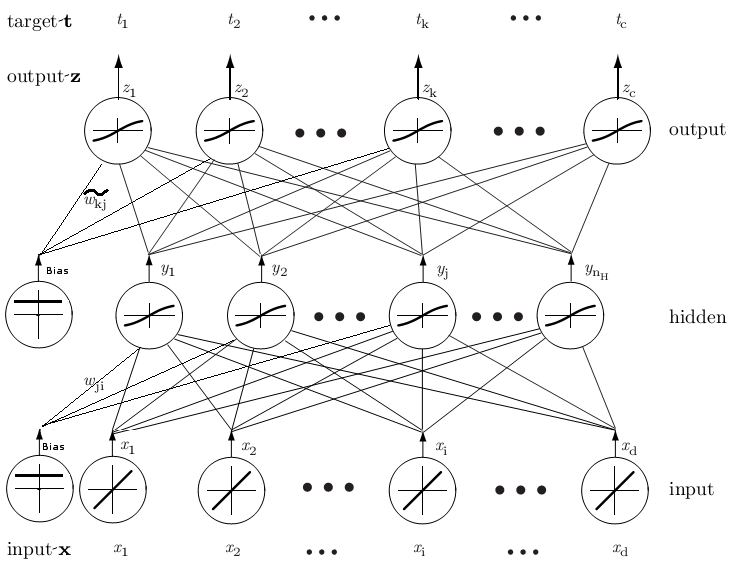
\includegraphics[width=10cm]{./images/feedforwardOperation.png}
 \end{minipage} 
 \hspace{5mm}
 \begin{minipage}{8cm}
  \textbf{Input Layer (x)}: Represent the input $\bm{ x}$ and has $d$ linear input nodes. 
  To standardize the inputs, the mean value of the training set has to be subtracted and it has to 
  be divided by its variance.\\
  \textbf{Output Layer (z)}: Represent the classes $\bm{ z}$ and has the dimension $c$. This nodes can have a nonlinear weight function.\\
  \textbf{Hidden Layer}: Between output and input. There can be more than one hidden layer. 
  Has most of the time non-linear weight function. The number of this nodes $n_H$ is a design parameter.\\
  \textbf{Modifiable weights/ Synapse} $\bm{ w_{ji}}$ and  $\bm{\tilde{w}_{kj}}$: 
  connect input $(i)$ with hidden $(j)$ node and hidden $(j)$ with the output $(k)$ node, respectively.  \\
  \textbf{Bias Unit}: Used to model a bias in each layer. One bias unit is connected to each layer except the input layer: 
  $\omega_{j0}$ input bias, $\tilde \omega_{k0}$ hidden bias.\\
  \textbf{Net Activation}: The sum of all weighted inputs of a node is called \em net activation \em or \em net\em. 
  $ net_j =\sum\limits_{i=0}^d x_i w_{ji} = \bm w_j^T\bm x$ for hidden nodes,
  $ \tilde{net}_k =\sum\limits_{j=0}^{n_H} y_j \tilde{w}_{kj} = \bm{ \tilde{w}}_k^T\bm y$ for output nodes.\\
 \end{minipage}\\
  \textbf{Activation Function (Neuron)}: Every node has an \em activation function $f(\cdot)$\em. 
  $y_j=f_j(net_j)$ for hidden nodes, $z_k=\tilde f_k(\tilde{net}_k)$ for output nodes.  
  The function $f_j$ and $\tilde f_k$ is usually the same and non-linear. 
  A common function for MNN is the sigmoid function $\bm{f=a \tanh(b \cdot net)}$.
  The input function $f_i$ is often linear. \\
  
  \textbf{Discriminant function}: The \em discriminant function \em is the sum of all nodes:
  $$ g_k(\bm x) \equiv z_k = \tilde f_k\left( \sum\limits_{j=1}^{n_H} \tilde{w}_{kj} \cdot f_j 
    \left( \sum\limits_{i=1}^d w_{ji} x_i +w_{j0} \right)+ \tilde{w}_{k0} \right) \qquad k=[1,\ldots,c]$$ 
  
  \textbf{Kolmogorov}: Kolmogorov showed that all function can be constructed with a three layer network and enough hidden nodes.
  
 \skriptsubsection{Backpropagation Algorithm}{288}
 The \em Backpropagation Algorithm \em is used to learn the network.
 The goal is again to minimize the error function $J( w, \tilde{w})=J(\bm w)\equiv \frac{1}{2}\| \bm t - \bm z \|^2 $ where $\bm t$ the is target vector. For numerical 
 reasonsoften the labeled class is often set to 1 the rest to -1, e.g. $\bm t =[1,-1,\ldots,-1]^T$. \\
 Because the algorithm is based on gradient descent, the weights are updated similarly:
 $\bm w(m+1)=\bm w(m)+\Delta \bm w(m)$ with $\Delta \bm w = -\eta \frac{\partial \bm J}{\partial \bm w}$\\
 \subsubsection{Backpropagation Process}
 \begin{minipage}{12cm}
 \begin{aufzaehlung}
   \item Initialize $\omega$ with uniformly distributed random values. \\
   Borders for $\omega_{ji}: \pm \frac{1}{\sqrt{d}}$, $\tilde \omega_{kj}: \pm \frac{1}{n_H}$
   \item Define target $\bm t$ of given training samples $\bm x $ ($t_k=1$, $t_{i \neq k} = -1$)
   \item Classify one training sample $\bm x$ by feedforward operation
   \item Calculate the \em output sensitivity \em $\tilde{\delta}_k \equiv (t_k - z_k) f'(\tilde{net}_k)$
   \item Update the weight vectors between hidden and output layer with:\\
   $ \Delta \tilde{w}_{kj} = \eta \title{\delta}_k y_j$
   \item Calculate the \em hidden sensitivity \em $\delta_j \equiv f'(net_j) \sum_{k=1}^c \tilde{w}_{kj}\tilde{\delta}_k$
   \item Update the weight vectors between input and hidden layer:\\
   $\Delta w_{ji}= \eta x_i \delta_j = \eta \left[ \sum\limits_{k=1}^c \tilde{w}_{kj} \tilde{\delta}_k \right] f'(net_j) x_i$
 \end{aufzaehlung}
 \end{minipage}
 %\hspace{5mm}
 \begin{minipage}{7.5cm}
 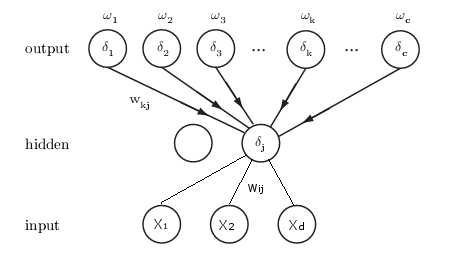
\includegraphics[width=7.5cm]{./images/backpropagation.png}
 \end{minipage}\\
 
 \begin{minipage}{8cm}
 \skriptsubsubsubsection{Variants}{293}
 \begin{liste}
   \item Input units include a bias unit. (very often)
   \item There are different non-linearities for different layers
   \item There are more than three layers. (the process works similar to the steps 3 \& 4)
   \item Input units are connected directly to output units as well as to hidden units
   \item Each unit has its own non-linearity
   \item Each unit has a different learning rate
 \end{liste}
 
 \end{minipage}
 \begin{minipage}{10cm}
 \skriptsubsubsubsection{Training Protocols}{293}\\
 There are different variant how to present the training set to the algorithm:\\
 \begin{liste}
   \item The \em Stochastic Training \em is the most common variant. The training sample are chosen randomly out of the training set\\
   \item In \em On-Line Training \em the training pattern are presented only once. So no memory for storing are used. An example of this variant is the frog algorithm from Guido\\
   \item The \em Batch training \em is not really common. Here all training data were presented before take one update.\\
 \end{liste}
 \end{minipage}
 
 \begin{minipage}{10cm}
 \skriptsubsubsubsection{Stopping Criterion}{295}\\
 To avoid overfitting, after every epoch (train all training sample one time) validation is done with a small set of data.
 This data set has to be separated from the training samples.
 If the validation is going to be worse, the training has to be stopped.\\
 
 After stopping a test has to decide if the result is good enough. For this a bigger data set (again separated from the training data) is tested and 
 the total error $\bm J = \sum\limits_{p=1}^n \bm J_p$ has to be low enough.
 \end{minipage}
 \hspace{5mm}
 \begin{minipage}{8cm}
 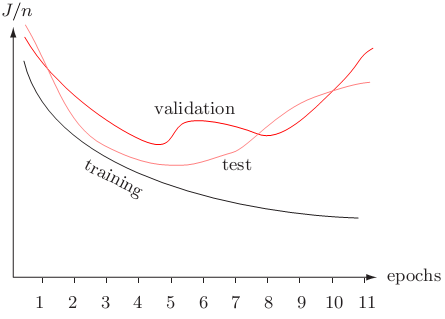
\includegraphics[width=7.5cm]{./images/stopCriterion.png}
 \end{minipage}
 
 \begin{minipage}{12cm}
 \skriptsubsection{Activation Function}{307}
 $$ f(net)=a \tanh(b \cdot net)= a \left[\frac{e^{b\cdot net}-e^{-b \cdot net}}{e^{b\cdot net}+ e^{-b\cdot net}}\right]$$
  The sigmoid is a function which is non-linear, continuous, differentiable, monotonous, smooth and saturating. Its maximum steepness is at 0.
  
  \skriptsubsubsection{Parameters}{308}
  It is important to choose the parameters for the sigmoid carefully. The factor $a$ defines the maximum output of an node.
  It should be bigger than the maximum of the needed output. A common value is $1.716$ if the output is normalized to $1$.
  If $a$ is to large, the sigmoid function is almost linear and if $a$ is to small, the function is in saturation and the target won't be reached or just to slowly.
  If $b=2/3$ is chosen, the maximum of the first derivation is 1 and and that the linear range is $\approx -1 < net < +1$ 
  \subsubsection{Scaling Input}
  The input (training and test samples) has often be scaled / standardize. The variance and the mean over \textbf{all} trainings sample should be: 
  $\sigma^2=1$ and $\mu=0$. The same factors as used for the training data has to be used for operation.
  
  
 \skriptsubsection{Techniques for Improving Backpropagation}{309}
 
 \end{minipage}
 \hspace{8mm}
 \begin{minipage}{5.6cm}
 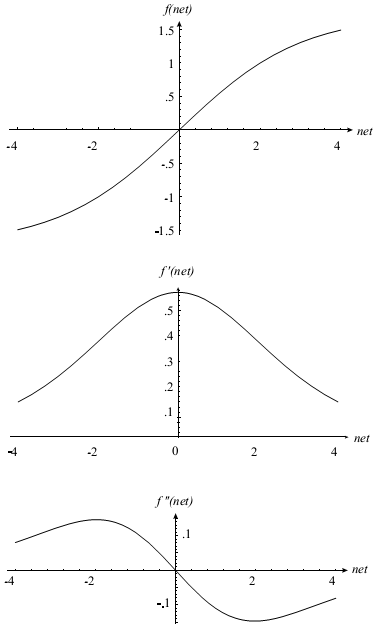
\includegraphics[width=5.6cm]{./images/sigmoid.png}
 \end{minipage} 
 
 \skriptsubsubsection{Training with Noise}{310}
 To have more training samples, the true training samples can be added with d-dimensional Gaussian noise.
 If the training samples were standardized the variance has to be less than 1 (e.g. 0.1) and the category label should be left unchanged.
 
 \skriptsubsubsection{Number of Hidden Units}{310}
 When the number of hidden units is too low, the performance is probably too low, but a high number 
 increases the danger of overfitting. A rule of thumb is $n_H = n/10$ with $n$ as the number of training samples.
 
 \skriptsubsubsection{Learning Rates}{312}
 The training rates $\eta$ does not have to be constant. In general,  $\eta < 2\eta_{opt}$ with $\eta_{opt}= \left( \frac{\partial^2\bm J}{\partial w^2} \right)^{-1}$ (Newton). 
 A first choice can be $\eta \approx 0.1$ or $\eta \approx 0.01$.
 
 \skriptsubsubsection{Momentum}{313}
 The momentum is a kind of lowpass filtering of the update direction. So not only the current update value is used also the last one:\\
 $\bm w(m+1)= \bm w(m) +(1-\alpha) \Delta\bm w_{bp}(m) + \alpha \Delta \bm w(m-1)$ with $\alpha \approx 0.9$.
 
 \skriptsubsubsection{Weight Decay}{314}
 Before updating the weight vectors they are made a bit smaller $\bm w_{new}= \bm _{old}(1-\epsilon)$. 
 This has the effect that rare (unimportant) but big samples slowly eliminated and the often/important but small vectors are counted more.
 
 \skriptsubsubsection{Hint}{315}
 The idea is to give during the training additional knowledge into the algorithm with additional output nodes. For the test this nodes are ignored. 
 One example could be the frog, where the training is also given in which quadrant the fly is.
 

 \skriptsubsection{Backpropagation as Feature Mapping (Kind of Voodoo)}{299}

 \skriptsubsection{Backpropagation, Bayes Theory and Probability}{303}
 Shows that neural networks approximate the \em a posteriori probability\em.
 
\newpage
\begin{landscape}
\section{Overview over Different Methods}
\begin{tabular}{| p{3cm} |  p{3.5cm} | p{5cm} | p{4cm} | p{8cm} |}
\hline
Name& 	Precondition & Idea & Design Parameter & Dis-/Advantages\\
\hline
\textbf{Bayes Decision Theory} &
	All  probability distributions with parameters are known &
	Results into the optimal decision &
	- &
	\begin{beschreibListe}
	\item[+] Optimal
	\item[-] All $P(\bm x | \omega_i)$ have to be known
	\end{beschreibListe}	\\
\hline
\textbf{Maximum-Likelihood} &
	All probability distributions without parameters, some trainings pattern &
	Estimate the distribution parameter so that $P(\mathcal D|\theta)$ is maximized&
	Model $p(\bm x | \theta)$ &
	\begin{beschreibListe}
	\item[+] Simple
	\item[-] Check for local maxim or worse minimum needed
	\item[-] No possibility to add prior knowledge
	\end{beschreibListe}\\
\hline
\textbf{Bayes Parameter Estimation} &
	All probability distributions without parameter, some training samples &
	Estimate the distribution of parameters with own probability density.   &
	\begin{beschreibListe}
	\item[-] Model of $p(\bm x|\bm \theta)$
	\item[-] Prior density $P(\bm \theta)$ form and parameter 
	\end{beschreibListe} &
	\begin{beschreibListe}
	\item[-] More complicated to calculate and understand
	\item[+] Better results with prior knowledge for $\bm \theta$
	\end{beschreibListe}\\
\hline
\textbf{Hidden Markov Model} &
	Sequence of training samples, known model of hidden states (without parameter) &
	Be able to model time dependencies. &
	Topology of hidden states &
	
	\begin{beschreibListe}
	\item[+] Be able to model time dependencies
	\end{beschreibListe} \\
\hline
\textbf{Parzen Window} &
	Enough training data &
	Estimate $p(\bm x | \omega_i)$ by convoluting each training samples $\bm X_t$ 
	with a given window $\varphi $ $\Rightarrow p(\bm x | \omega_i) \approx \sum \bm X_t \ast \varphi $ &
	Window function, \textbf{width of the window function} $V_n / h_n$ &
	
	\begin{beschreibListe}
	\item[-] Needs a lot of calculation to evaluate test pattern
	\item[+] No knowledge about the distribution needed
	\item[+] Easy to learn (PNN)
	\item[+] Convergent to $p(x|\omega)$
	\item[+] Easy to parallelize
	\end{beschreibListe}   \\
\hline
\textbf{k-Nearest Neighbor} &
	Enough training data &
	Estimate $P(\omega_i|\bm x)$ directly, ``choose the class of which the most pattern are around me'' &
	\textbf{Number of samples } $(k_n)$, Metric &
	\begin{beschreibListe}
	\item[+] Needs less calculation to evaluate test patten than Parzen Window
	\item[+] Easy to understand
	\item[-] Metric relevant
	\item[-] Does not converge to Bayes (worst case factor 2 away)
	\end{beschreibListe}\\
\hline
\textbf{Linear Discriminant Functions} &
	Training samples (the more the better), data should be (almost) linear separable &
	Search a separable hyperplane (defined with a weight vector $\bm a$), no estimation of $p(\bm x |\omega) / p(\omega | \bm x)$ &
	Training algorithm, step size $(\eta)$, margin $b$, possible feature mapping into non-linear space $(x, x^2, yx, \ldots)$ &
	
	\begin{beschreibListe}
	\item[+] Only training is complex 
	\item[+] Good generalization because of linear
	\item[-] Long training time
	\item[-] Works only if the data are more or less linear separable
	\end{beschreibListe} \\
\hline
\textbf{Multilayer Neural Network} & 
	Many, many training samples &
	The nonlinear feature mapping should be self learning, with a three layer network all distribution can be built theoretically. &
	Network topology (\# layers, \# hidden nodes, special stuff (feedback, etc)), activation function &
	
	\begin{beschreibListe}
	\item[+] No prior knowledge are needed
	\item[+] Easy to add constraints
	\item[-] Much training data needed
	\item[-] Sometimes too many degrees of freedom
	\item[-] Long training time
	\end{beschreibListe}\\
\hline

	
\end{tabular}

\end{landscape}

\end{document}
